\documentclass[11pt,a4paper,oneside]{report}
\usepackage[utf8]{inputenc}
\usepackage[T1]{fontenc}
\usepackage{lmodern}
\usepackage[english]{babel}
\usepackage[margin=2.6cm]{geometry}
\usepackage{amsmath,amssymb}
\usepackage{booktabs}
\usepackage{graphicx}
\usepackage{xcolor}
\usepackage{tikz}
\usetikzlibrary{arrows.meta,positioning,calc,shapes.geometric,fit,backgrounds,decorations.pathreplacing}
\usepackage[colorlinks=true,linkcolor=blue!50!black,citecolor=green!40!black,urlcolor=blue!50!black]{hyperref}
\graphicspath{{figures/}{../figures/}{../slides/}}

\definecolor{ink}{HTML}{14212B}
\definecolor{muted}{HTML}{586A77}
\definecolor{sky}{HTML}{2F6DB0}
\definecolor{climb}{HTML}{17936A}
\definecolor{sink}{HTML}{C9502F}
\definecolor{therm}{HTML}{E39A2D}

\tikzset{
  blk/.style={draw=muted, rounded corners=3pt, fill=white, align=center, font=\small, minimum height=1.0cm, inner sep=5pt},
  key/.style={blk, draw=climb, line width=1pt},
  arr/.style={-{Stealth[length=2.2mm]}, draw=muted, line width=0.7pt},
  lab/.style={font=\scriptsize, text=muted, align=center},
}
\newcommand{\vect}[1]{\boldsymbol{#1}}
\newcommand{\R}{\mathbb{R}}
\newcommand{\E}{\mathbb{E}}
\newcommand{\CL}{C_L}
\newcommand{\CLmax}{C_{L,\max}}

\title{\textbf{GeneticWing}\\[0.6em]\Large Learning to Soar:\\ Evolutionary Search in Learned Spaces, Physics-Informed Generative Planning and Distillation for Fixed-Wing UAV Soaring}
\author{Clément Dumeril}
\date{Research report, November 2026}

\begin{document}
\maketitle

\begin{abstract}
Fixed-wing drones can extend their endurance by harvesting energy from rising air, as sailplane pilots do, but planning energy-optimal trajectories through thermals is a non-convex, multimodal problem whose good solutions sit against stall and load limits. This report studies how to make such planning both good and fast. A point-mass, differentially flat model of a 4.2\,kg motor-glider (SB-XC), refined with a strip-theory wing that captures inner-wing stall in turns, turns any candidate trajectory into lift coefficient, bank and required thrust without integration. A slow offline \emph{teacher} (a reactive orbit law tuned by a genetic algorithm, fitted and refined by sequential quadratic programming) solves 15{,}080 randomized single-thermal situations. A conditional variational autoencoder whose decoder outputs bounded \emph{commands} flown by a differentiable simulator compresses those solutions into a 16-dimensional latent space; a genetic algorithm searching that space beats its own teacher by 0.84 energy units (cost $-5.72$ against $-4.88$ on 65 held-out situations), whereas the same algorithm on the raw 87-dimensional trajectory genome was the weakest optimizer tested. Flown in closed loop by an autopilot in turbulent air with model-predictive replanning, the advantage holds in calm air; the dominant loss is an error on the thermal's position. On 64 cross-country tasks of 20\,km, a MacCready tactician whose climbs are flown by the latent genetic search climbs 61\,\% faster than a classic circling rule and matches the speed of motorized flight with 13 times less battery, without any stall once an inner-wing limiter is added to the autopilot. Finally, the search is distilled into a conditional flow-matching generator; after one DAgger round on the states met in flight, it plans in 0.24\,s instead of 13\,s and climbs at 2.23\,m/s, as well as the search it imitates. The report details the models, algorithms and results, the failures that shaped them, and the path to a flight test on a laboratory airframe.
\end{abstract}

\tableofcontents
\listoffigures
\listoftables

%=====================================================================
\chapter{Introduction}

\section{Motivation}
Small fixed-wing UAVs are limited by their battery. Gliders show the alternative: the atmosphere is full of rising air (thermals, ridge lift, wind shear), and a pilot who knows where to circle can stay aloft for hours without a motor. Autonomous soaring has been demonstrated in flight, notably with the SB-XC sailplane at the US Naval Research Laboratory \cite{edwards2008}, and recent work on differentially flat fixed-wing planning \cite{morando2025,morando2026} has made energy-aware trajectory planning fast enough for onboard replanning, but stops short of harvesting energy.

Planning to soar is hard for three reasons. The objective (net energy over a horizon) is non-convex and multimodal: a thermal can be circled clockwise or counter-clockwise, entered from several sides, at several radii. The best trajectories sit on constraints (lift coefficient near stall, bank and load limits), so any approximation error makes them infeasible. And the problem must be solved again every few seconds in flight, because the air never matches the plan.

\section{Research question and hypotheses}
\begin{quote}\itshape
Can a generative model trained to imitate an offline optimizer propose near-optimal soaring trajectories fast enough for onboard replanning, once checked by the physics and refined by local optimization?
\end{quote}
The question was broken into six hypotheses, whose verdicts are summarized in Table~\ref{tab:hypotheses} and argued in the following chapters.

\begin{table}[ht]\centering\small
\caption{Hypotheses and verdicts.}\label{tab:hypotheses}
\begin{tabular}{@{}p{0.3\linewidth}p{0.17\linewidth}p{0.45\linewidth}@{}}
\toprule
Hypothesis & Verdict & Evidence \\ \midrule
H1: a genetic algorithm (GA) is a good offline teacher & rejected, then reformulated & weakest optimizer on the 87-gene genome (Ch.~\ref{ch:teacher}); best method when searching a learned latent space (Ch.~\ref{ch:student}) \\
H2: a student plans in real time near the optimum & supported in the end & flow matching on genomes keeps $\approx$40\,\% of the gain; the distilled latent generator matches the GA in 0.24\,s (Ch.~\ref{ch:distill}) \\
H3: generative beats regression (multimodality) & supported & regression averages the two orbit directions into an infeasible straight line \\
H4: physics check + local refinement close the gap & partly & student-seeded NLP solves 76\,\% vs 8\,\% from straight flight \\
H5: robustness to wind errors and gusts & open & holds in calm air; a 15\,m error on the thermal centre halves the gain (Ch.~\ref{ch:closedloop}) \\
H6: self-improvement loop & supported once & first loop on position genomes: no gain; DAgger round on flight states: large gain (Ch.~\ref{ch:distill}) \\
\bottomrule
\end{tabular}
\end{table}

\section{Contributions}
\begin{enumerate}
  \item A flat, vectorized evaluation of soaring trajectories with a strip-theory wing, a unified energy cost and constraint handling for motor-gliders (Ch.~\ref{ch:model}).
  \item Evidence that representation decides whether evolutionary search works: the same GA fails on raw trajectories and beats its teacher in the latent space of a physics-informed decoder (Ch.~\ref{ch:student}).
  \item A command-space VAE whose decoder is a differentiable simulator, making every decoded plan dynamically feasible by construction (20\,\% to 100\,\% round-trip feasibility).
  \item A closed-loop evaluation with an autopilot, turbulence and wrong beliefs, and the model-predictive ingredients that make replanning safe (shrinking horizon, warm start, state continuity) (Ch.~\ref{ch:closedloop}).
  \item A two-level cross-country pilot (MacCready tactician, planned climbs) and an inner-wing stall limiter, evaluated on 64 tasks of 20\,km (Ch.~\ref{ch:xc}).
  \item A distillation of the search into a flow-matching generator, corrected by DAgger on flight states, that plans in 0.24\,s with the quality of the search (Ch.~\ref{ch:distill}).
\end{enumerate}

\begin{figure}[ht]\centering
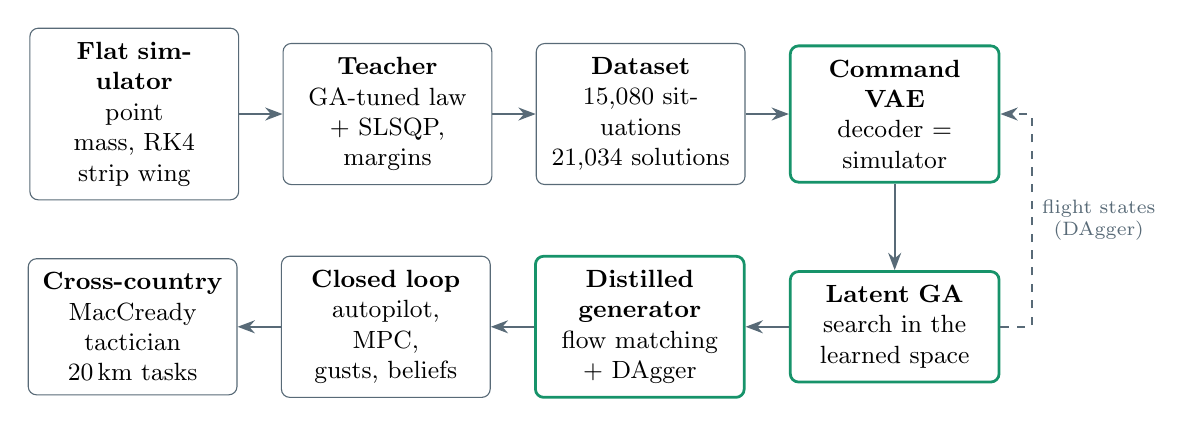
\begin{tikzpicture}[node distance=0.55cm]
  \node[blk, text width=2.3cm] (sim) {\textbf{Flat simulator}\\point mass, RK4\\strip wing};
  \node[blk, text width=2.3cm, right=of sim] (teach) {\textbf{Teacher}\\GA-tuned law\\+ SLSQP, margins};
  \node[blk, text width=2.3cm, right=of teach] (data) {\textbf{Dataset}\\15{,}080 situations\\21{,}034 solutions};
  \node[key, text width=2.3cm, right=of data] (vae) {\textbf{Command VAE}\\decoder = simulator};
  \node[key, text width=2.3cm, below=1.1cm of vae] (ga) {\textbf{Latent GA}\\search in the\\learned space};
  \node[key, text width=2.3cm, left=of ga] (dis) {\textbf{Distilled}\\\textbf{generator}\\flow matching + DAgger};
  \node[blk, text width=2.3cm, left=of dis] (cl) {\textbf{Closed loop}\\autopilot, MPC,\\gusts, beliefs};
  \node[blk, text width=2.3cm, left=of cl] (xc) {\textbf{Cross-country}\\MacCready tactician\\20\,km tasks};
  \draw[arr] (sim) -- (teach); \draw[arr] (teach) -- (data); \draw[arr] (data) -- (vae);
  \draw[arr] (vae) -- (ga); \draw[arr] (ga) -- (dis); \draw[arr] (dis) -- (cl); \draw[arr] (cl) -- (xc);
  \draw[arr, dashed] (ga.east) -- ++(0.4,0) |- node[lab, pos=0.25, right]{flight states\\(DAgger)} (vae.east);
\end{tikzpicture}
\caption{The GeneticWing pipeline. Green boxes are the learned components.}\label{fig:pipeline}
\end{figure}

\section{Outline}
Chapter~\ref{ch:background} reviews the background. Chapter~\ref{ch:model} presents the physical model. Chapters~\ref{ch:teacher} to \ref{ch:distill} follow the six phases of the work: the teacher, the generative students and the latent search, the closed loop, cross-country flight, and the distillation of the search. Chapter~\ref{ch:discussion} discusses the findings and their limits, Chapter~\ref{ch:towards} the path to a flight test, and Chapter~\ref{ch:conclusion} concludes.

%=====================================================================
\chapter{Background}\label{ch:background}

\section{Soaring flight}
\paragraph{Thermals.} A thermal is a column of warm rising air. Allen's model \cite{allen2006} scales the mean updraft $\bar w(z)$ and the outer radius $r_2(z)$ with the convective velocity $w^\star$ and the boundary-layer depth $z_i$:
\begin{equation}
\bar w(z) = w^\star \Big(\frac{z}{z_i}\Big)^{1/3}\Big(1 - 1.1\frac{z}{z_i}\Big), \qquad
r_2(z) = \max\!\Big(10,\; 0.102\Big(\frac{z}{z_i}\Big)^{1/3}\Big(1-0.25\frac{z}{z_i}\Big) z_i\Big).
\end{equation}
We use a Gaussian core of radius $r_2/2$ whose disk mean equals $\bar w$; the core drifts with the horizontal wind (Fig.~\ref{fig:thermal}). At 250\,m altitude the core radius is about 30\,m: a 15\,m error on its position is large.

\begin{figure}[ht]\centering
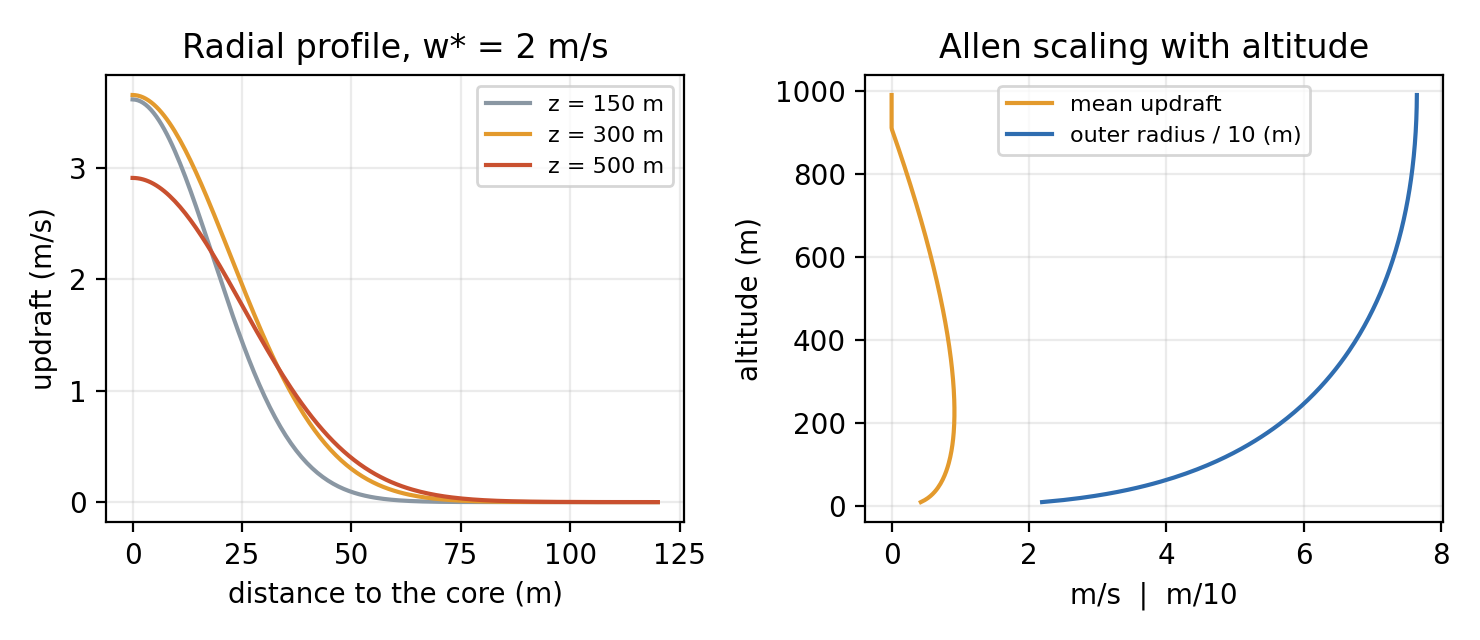
\includegraphics[width=0.92\linewidth]{thermal_model.png}
\caption{Thermal model: radial updraft profile at three altitudes, and Allen's vertical scaling.}\label{fig:thermal}
\end{figure}

\paragraph{MacCready theory.} Cross-country pilots alternate climbs in thermals and glides between them. MacCready \cite{maccready1958} showed that, expecting to climb at rate $M$ in the next thermal, the airspeed that maximizes the average cross-country speed minimizes the time per unit distance including the climb:
\begin{equation}\label{eq:stf}
V^\star(M, w) = \arg\min_V \frac{s(V) - w + M}{V},
\end{equation}
with $s(V)$ the still-air sink rate and $w$ the vertical air motion. Geometrically, $V^\star$ is the tangent to the polar from the point $(0, M)$ (Fig.~\ref{fig:polar}). The same reasoning tells the pilot to leave a thermal once its climb falls below $M$.

\begin{figure}[ht]\centering
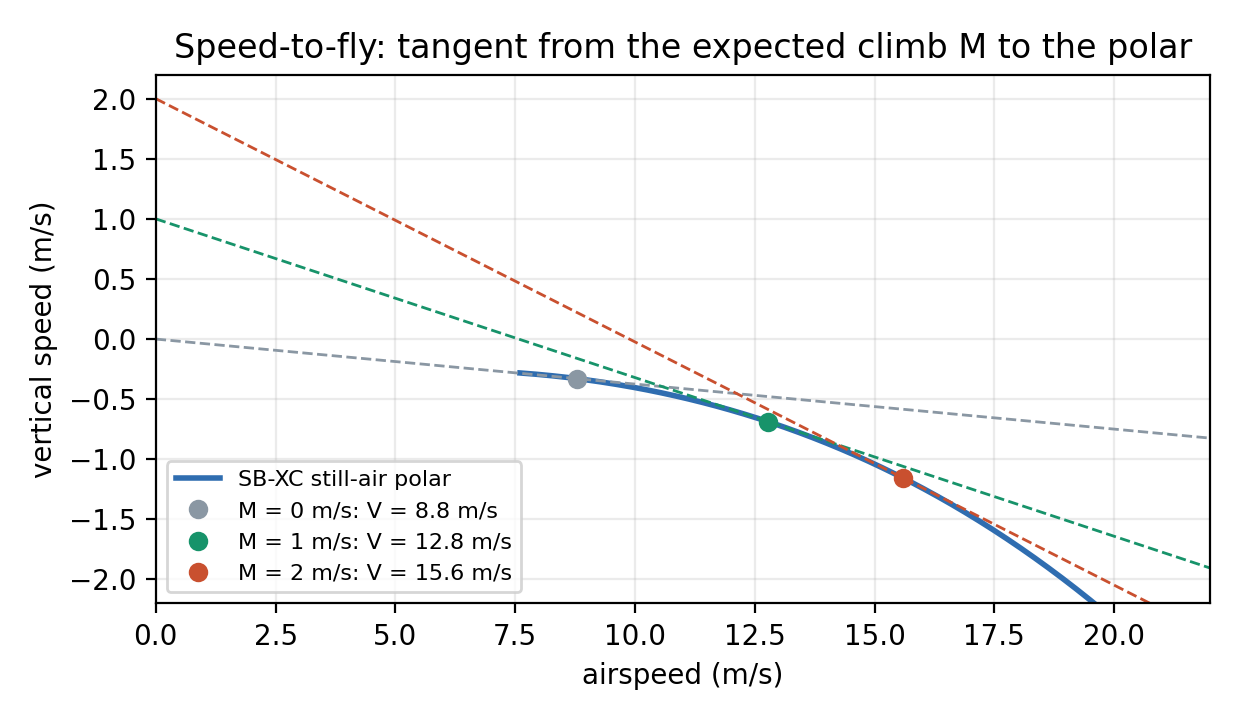
\includegraphics[width=0.72\linewidth]{polar_maccready.png}
\caption{SB-XC polar and MacCready speed-to-fly construction.}\label{fig:polar}
\end{figure}

\section{Differential flatness of the coordinated fixed wing}
For a point mass in coordinated flight with inputs (lift coefficient $\CL$, bank $\phi$, thrust $T$), the position $\vect p(t)$ together with the wind $\vect W(\vect p,t)$ determines every other state and input algebraically \cite{morando2025}. This is the flat map used throughout (Section~\ref{sec:flat}). Without a motor, position is no longer a flat output: a glider has two inputs for three outputs; the planner then imposes $T_{\mathrm{req}} = 0$ as a constraint, which generalizes the sink-rate constraint of \cite{morando2026} to non-uniform wind.

\section{Optimization}
\paragraph{Genetic algorithms.} A real-coded GA evolves a population of candidate vectors with simulated binary crossover (SBX) \cite{deb1995} and polynomial mutation. With constraints, Deb's feasibility rules \cite{deb2000} rank feasible solutions by cost and infeasible ones by total violation, feasible first. We also use the GA of T.~Zohdi's course (80\,\% random immigrants per generation) to tune a 10-parameter reactive law, and CMA-ES \cite{hansen2001} as a reference.
\paragraph{Local optimization.} Sequential least-squares quadratic programming (SLSQP) \cite{kraft1988} refines a candidate under constraints, with finite-difference gradients evaluated in one vectorized batch.
\paragraph{Constraint aggregation.} Time-series constraints $g_k(t)\le 0$ are aggregated with the Kreisselmeier--\-Steinhauser (KS) function \cite{ks1979}
\begin{equation}
\mathrm{KS}(g) = \max_t g + \frac{1}{\rho}\log\sum_t e^{\rho (g(t) - \max_t g)},
\end{equation}
a smooth, conservative maximum (by at most $\log N/\rho$).

\section{Generative models}
\paragraph{Variational autoencoders.} A conditional VAE \cite{kingma2014} encodes a solution $\vect x$ given a context $\vect c$ into a latent $\vect z$ and decodes it back, trained on the evidence lower bound
\begin{equation}
\mathcal L = \E_{q(\vect z\mid\vect x,\vect c)}\big[\log p(\vect x\mid\vect z,\vect c)\big] - \beta\,\mathrm{KL}\big(q(\vect z\mid\vect x,\vect c)\,\|\,\mathcal N(0,I)\big).
\end{equation}
\paragraph{Flow matching.} Conditional flow matching \cite{lipman2023} with straight paths (rectified flow \cite{liu2023}) learns a velocity field $v_\theta$ that transports noise $\vect x_0\sim\mathcal N(0,I)$ to data $\vect x_1$:
\begin{equation}\label{eq:fm}
\mathcal L_{\mathrm{FM}} = \E_{t,\vect x_0,\vect x_1}\big\| v_\theta\big((1-t)\vect x_0 + t\vect x_1,\, t,\, \vect c\big) - (\vect x_1 - \vect x_0)\big\|^2,
\end{equation}
and samples by integrating $\dot{\vect x} = v_\theta(\vect x, t, \vect c)$ from $t=0$ to $1$ in a few Euler steps. Because it models a distribution, it can represent both orbit directions instead of averaging them.
\paragraph{Latent variable evolution.} Searching the latent space of a generative model with an evolutionary algorithm \cite{volz2018,gaier2020} replaces a high-dimensional, coupled search by a low-dimensional one over plausible solutions.

\section{Imitation and expert iteration}
Behaviour cloning trains on the expert's state distribution and fails when the learner visits states the expert never did. DAgger \cite{ross2011} aggregates data on the learner's own state distribution, labelled by the expert. Expert iteration \cite{anthony2017} and AlphaZero \cite{silver2018} alternate a slow search that improves on a policy and a network trained to reproduce the search's output. Chapter~\ref{ch:distill} applies both ideas to the latent genetic search.

%=====================================================================
\chapter{Modelling}\label{ch:model}

\section{Aircraft}
\begin{table}[ht]\centering\small
\caption{SB-XC model (C\textsubscript{D0}, $\CLmax$ and Oswald factor are estimates, tested at $\pm$20\,\% in Section~\ref{sec:sensitivity}).}\label{tab:aircraft}
\begin{tabular}{@{}lr@{\qquad}lr@{}}
\toprule
Mass & 4.22\,kg & Wing area & 1.07\,m\textsuperscript{2} \\
Span & 4.6\,m & Aspect ratio & 19.8 \\
Max lift-to-drag ratio & 27.1 & Min-drag airspeed & 8.05\,m/s \\
$\CLmax$ & 1.2 & Motor (motor-glider conversion) & 15\,N \\
Propulsive efficiency & 0.5 & Polar & parabolic, $C_D = C_{D0} + k\CL^2$ \\
\bottomrule
\end{tabular}
\end{table}

\section{Point-mass dynamics}
In the inertial frame (east, north, up), with air velocity $\vect v_a = \vect v - \vect W(\vect p,t)$, airspeed $V_a = \|\vect v_a\|$ and dynamic pressure $q = \tfrac12\rho V_a^2$,
\begin{equation}\label{eq:dyn}
m\dot{\vect v} = q S \CL\big(\cos\phi\,\hat{\vect u}_\perp + \sin\phi\,\hat{\vect r}\big) + \big(T - qS\,C_D(\CL)\big)\hat{\vect v}_a - m g\,\hat{\vect e}_z,
\end{equation}
with $\hat{\vect v}_a$ the unit air velocity, $\hat{\vect u}_\perp$ the unit vector normal to it in the vertical plane and $\hat{\vect r} = \hat{\vect v}_a\times\hat{\vect u}_\perp$ the right-wing direction (Fig.~\ref{fig:forces}).

\begin{figure}[ht]\centering
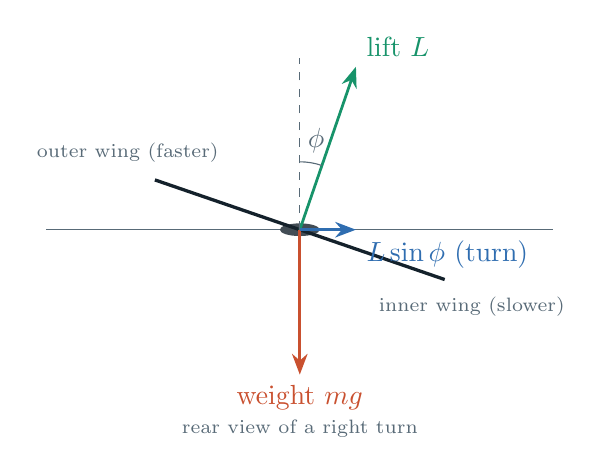
\begin{tikzpicture}[scale=1.15]
  \draw[muted, thin] (-2.8,0) -- (2.8,0);
  \fill[ink!80] (0,0) ellipse (0.22 and 0.07);
  \draw[ink, line width=1.2pt] (-1.6,0.55) -- (1.6,-0.55);
  \draw[-{Stealth}, line width=1pt, climb] (0,0) -- (0.62,1.8) node[above right]{lift $L$};
  \draw[-{Stealth}, line width=1pt, sink] (0,0) -- (0,-1.6) node[below]{weight $mg$};
  \draw[-{Stealth}, line width=1pt, sky] (0,0) -- (0.62,0) node[below right]{$L\sin\phi$ (turn)};
  \draw[dashed, muted] (0,0) -- (0,1.9);
  \draw[muted] (0,0.75) arc (90:71:0.75); \node[muted] at (0.18,0.98) {$\phi$};
  \node[lab] at (-1.9,0.85) {outer wing (faster)};
  \node[lab] at (1.9,-0.85) {inner wing (slower)};
  \node[lab] at (0,-2.2) {rear view of a right turn};
\end{tikzpicture}
\caption{Forces in a banked, coordinated turn. The horizontal component of lift turns the aircraft; the inner wing flies slower than the outer one.}\label{fig:forces}
\end{figure}

\section{The flat map}\label{sec:flat}
Given a trajectory $\vect p(t)$ and its derivatives, $\vect v = \dot{\vect p}$ and $\vect a = \ddot{\vect p}$, the force the airframe must produce is $\vect F = m(\vect a + g\hat{\vect e}_z)$. Its component normal to $\vect v_a$ is the lift, and its axial component balances thrust and drag:
\begin{align}
\vect L &= \vect F - (\vect F\cdot\hat{\vect v}_a)\,\hat{\vect v}_a, \qquad \CL = \frac{\|\vect L\|}{qS}, \qquad n = \frac{\|\vect L\|}{mg},\\
\phi &= \operatorname{atan2}\big(\vect L\cdot\hat{\vect r},\; \vect L\cdot\hat{\vect u}_\perp\big), \qquad
T_{\mathrm{req}} = \vect F\cdot\hat{\vect v}_a + qS\,C_D(\CL).
\end{align}
No integration is needed: a population of trajectories, each sampled at 150 instants, is scored in one vectorized pass. $T_{\mathrm{req}}<0$ means excess energy that must be stored or bled.

\section{Trajectory parameterization}
Trajectories are clamped B-splines (chains of Bernstein polynomials) of degree 5 with 32 control points. The first three control points impose the initial position, velocity and acceleration; the 29 free ones are encoded ``turtle-style'' by a turn rate, a ground speed and a path angle per step, so that the genome has $3\times 29 = 87$ genes with physical bounds (turn rate $\le 30^\circ$/s, climb angle $\le 12^\circ$, ground speed 4--22\,m/s).

\section{Energy cost}
The cost is the net onboard energy over the horizon, normalized by the energy of level cruise on the motor at the best lift-to-drag speed:
\begin{equation}\label{eq:cost}
J = \frac{1}{E_{\mathrm{ref}}}\left(\int_0^H \frac{\max(T_{\mathrm{req}},0)\,V_a}{\eta}\,dt \;-\; \frac{m g\,\Delta e}{\eta}\right), \qquad
e = z + \frac{V_a^2}{2g}, \qquad E_{\mathrm{ref}} = \frac{mg}{(L/D)_{\max}}\,\frac{V_{md}\,H}{\eta}.
\end{equation}
$J = 1$ means cruising on the motor, $J<0$ net energy gained from the air ($J=-5$: five times the energy of a minute of motor cruise gained in a minute).

\section{Constraints and margins}
Hinge functions, positive when violated, cover thrust and braking capacity, $\CL\le 0.9\,\CLmax$, airspeed, bank $\le 45^\circ$, load factor $\le 2.5$, altitude, mission area, and with the strip wing, section stall and aileron authority. The teacher solves with \emph{tightened} constraints (constraint tightening, as in robust MPC): $\CL\le 0.75\,\CLmax$, bank $\le 38^\circ$, load $\le 2.1$, thrust $\le 0.8\,T_{\max}$; its solutions are scored under the nominal ones. Optimal solutions sit on their active constraints, and without margins any imitation error breaks them.

\section{Strip-theory wing}
\begin{figure}[ht]\centering
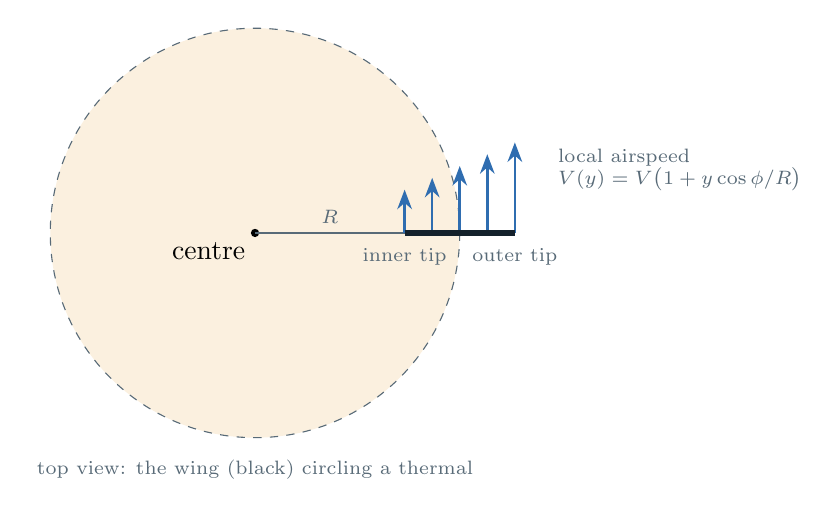
\begin{tikzpicture}[scale=1.0]
  \fill[therm!15] (0,0) circle (2.6);
  \draw[muted, dashed] (0,0) circle (2.6);
  \fill (0,0) circle (1.5pt) node[below left]{centre};
  \draw[muted] (0,0) -- node[above, lab]{$R$} (1.9,0);
  \foreach \r/\len in {1.9/0.55, 2.25/0.7, 2.6/0.85, 2.95/1.0, 3.3/1.15} {
    \draw[-{Stealth}, sky, line width=0.9pt] (\r,0) -- ++(0,\len);
  }
  \draw[ink, line width=2.4pt] (1.9,0) -- (3.3,0);
  \node[lab, align=left] at (5.4,0.8) {local airspeed\\$V(y) = V\big(1 + y\cos\phi / R\big)$};
  \node[lab] at (1.9,-0.3) {inner tip};
  \node[lab] at (3.3,-0.3) {outer tip};
  \node[lab] at (0,-3.0) {top view: the wing (black) circling a thermal};
\end{tikzpicture}
\caption{Strip theory in a turn. Each of 40 strips flies at its own airspeed; the slower inner wing reaches its section stall before the mean wing does.}\label{fig:strip}
\end{figure}
In a steady turn of radius $R$, a strip at spanwise position $y$ flies at $V(y) = V(1 + y\cos\phi/R)$. Holding the bank requires the ailerons to add lift on the slower inner wing, so the inner sections reach their stall coefficient first, the ailerons can run out of authority, and their deflection adds drag. With 40 strips, the minimum steady turn radius at 9\,m/s rises from 9\,m (point mass) to 18\,m, and the absolute minimum is about 11\,m at 10.5\,m/s (Fig.~\ref{fig:turnlimits}).

\begin{figure}[ht]\centering
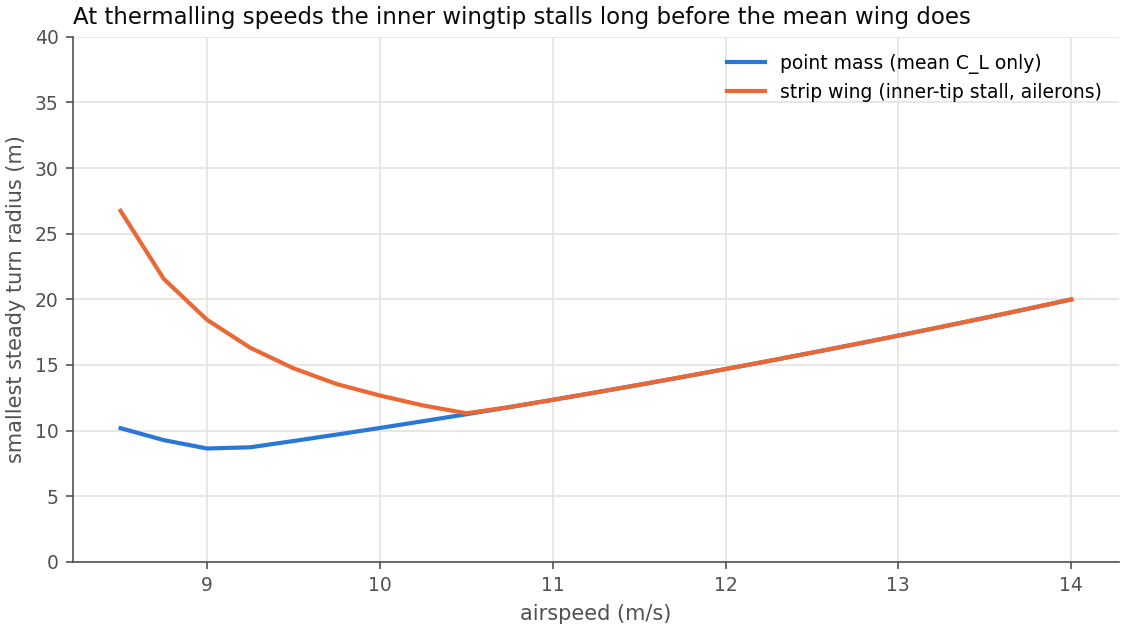
\includegraphics[width=0.7\linewidth]{turn_limits.png}
\caption{Minimum steady turn radius against airspeed: point mass and strip-theory wing.}\label{fig:turnlimits}
\end{figure}

\section{Integration: a lesson}
Simulated flights (the reactive law, the physics decoder, the closed loop) integrate equation~\eqref{eq:dyn}. With explicit Euler, a step that turns the velocity by lift adds energy:
\begin{equation}
\|\vect v + \vect a\,\Delta t\|^2 = \|\vect v\|^2 + 2\,\vect v\cdot\vect a\,\Delta t + \|\vect a\|^2\Delta t^2,
\end{equation}
and in a turn $\vect v\cdot\vect a\approx 0$, so every step injects $\|\vect a\|^2\Delta t^2$. A genetic search on the physics decoder found and exploited this free energy, reaching costs three times better than the teacher. All simulators now use the classical fourth-order Runge--Kutta scheme; a steady glide turn then loses exactly the polar's sink rate even with 0.4\,s steps. \emph{A powerful optimizer coupled to a simulator finds the simulator's flaws before it finds the physics.}

%=====================================================================
\chapter{The teacher}\label{ch:teacher}

\section{Phase 1: reproducing the ARPL glide}
Scenario S0 reproduces the straight glide of \cite{morando2026}: a 400\,m leg from 120\,m with a 12.5\,m/s airspeed reference and a 5.2\,m/s tailwind, flown in closed loop through 50 Dryden turbulence realizations \cite{milf8785c}. The error statistics of the real flight are recovered (Table~\ref{tab:s0}); the planner converges from 20 of 20 perturbed initial guesses.

\begin{table}[ht]\centering\small
\caption{Scenario S0: reproduction of the ARPL glide.}\label{tab:s0}
\begin{tabular}{@{}lccc@{}}
\toprule
Metric & ARPL flight & Plan, uniform wind & Closed loop, Dryden \\ \midrule
Mean airspeed (m/s) & 12.50 & 12.50 & 12.61 \\
Mean sink rate (m/s) & 1.48 & 1.58 & 1.61 \\
Glide ratio & 9.83 & 11.15 & 11.27 \\
Airspeed RMSE (m/s) & 1.09 & 0.00 & 0.87 \\
Netto RMSE (m/s) & 0.69 & 0.00 & 0.71 \\
\bottomrule
\end{tabular}
\end{table}

\section{Phase 2: which teacher?}
Eleven methods were compared at equal budget on three scenarios (S1 single thermal, S2 thermal field to a goal, S3 ridge lift), three instances each (Table~\ref{tab:phase2}).

\begin{table}[ht]\centering\small
\caption{Phase 2: mean cost of feasible solutions (20{,}000 evaluations; lower is better).}\label{tab:phase2}
\begin{tabular}{@{}lccc@{}}
\toprule
Method & S1 thermal & S2 field to goal & S3 ridge \\ \midrule
SLSQP from straight flight & $-2.77$ & infeasible & $-2.11$ \\
Real-coded GA (tuned, population 50) & $0.15$ & infeasible & $-0.73$ \\
Zohdi GA & infeasible & infeasible & infeasible \\
CMA-ES + SLSQP & $-3.80$ & infeasible & $\mathbf{-2.16}$ \\
GA, 100k evaluations & $-0.99$ & $0.47$ & $-1.83$ \\
Reactive law (Zohdi-tuned) & $-4.58$ & $\mathbf{-0.02}$ & $-1.96$ \\
\textbf{Law + SLSQP} & $\mathbf{-6.04}$ & infeasible & $-0.03$ \\
\bottomrule
\end{tabular}
\end{table}

\begin{figure}[ht]\centering
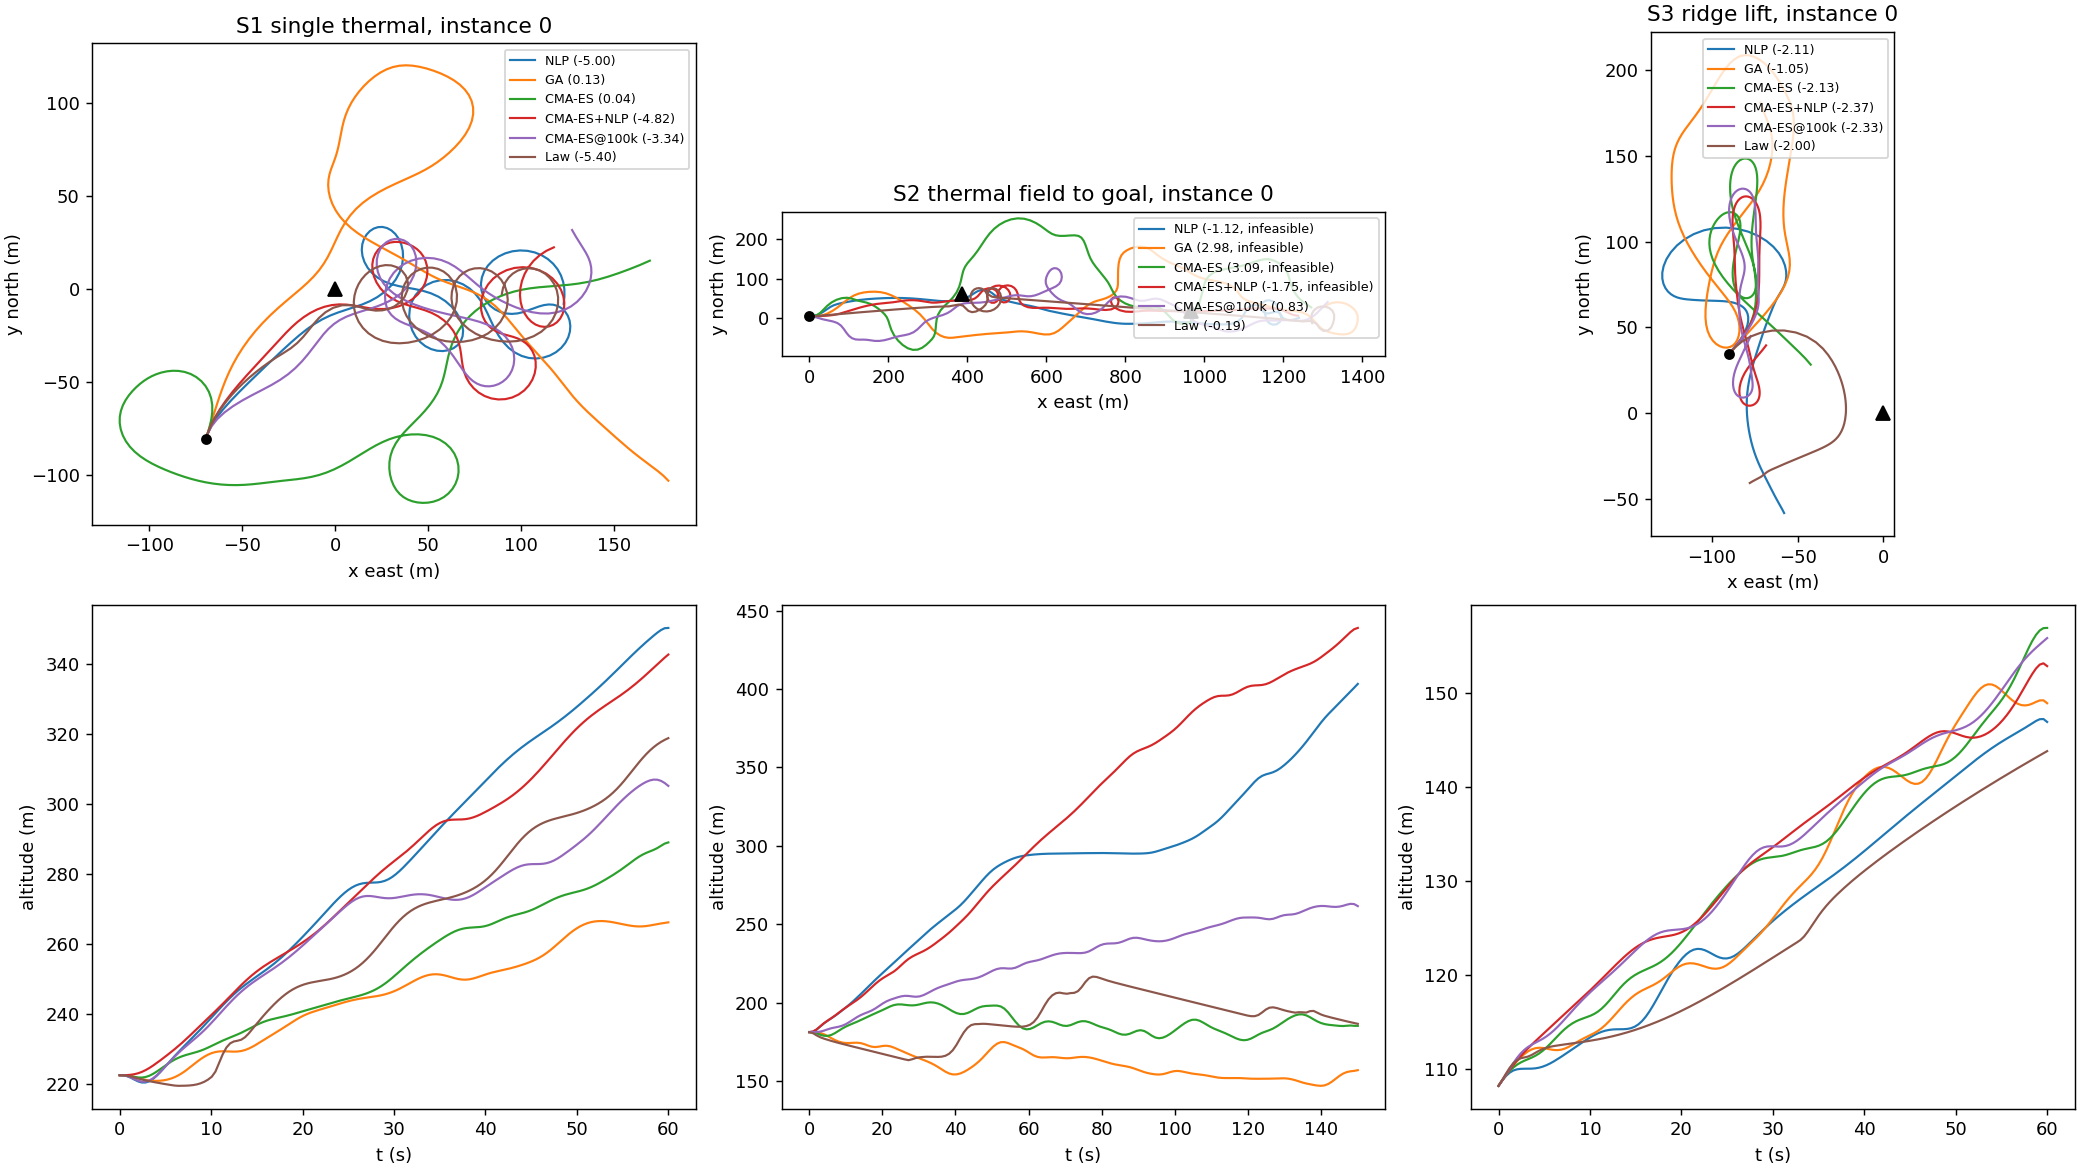
\includegraphics[width=0.95\linewidth]{phase2_trajectories.png}
\caption{Phase 2: trajectories of the best methods on S1, S2 and S3, and convergence.}\label{fig:phase2}
\end{figure}

H1 is not supported as stated: on 87 coupled genes the GA is the weakest working optimizer. \emph{Structure beats search}: a reactive orbit law (circle a centre at a given radius and speed, trade height for speed, motor below a floor) encodes the orbit the planners must otherwise discover. Fitting a genome to the law's flight and refining it by SLSQP gives the best teacher on S1 ($-6.04$, 30\,\% more energy than the law alone).

\section{The teacher at scale}
The randomized family S1 draws a thermal ($w^\star\in[1.2,2.8]$\,m/s), a wind (0--4\,m/s, any direction) and a start (60--200\,m from the thermal, 180--320\,m altitude, any heading). Each situation is solved in both orbit directions. On Savio (UC Berkeley), 21 nodes of 32 cores solve 15{,}080 situations in about 15 minutes.

\paragraph{Unsolved situations under the strip wing.} With the strip wing and the margins, the teacher left 39\,\% of the situations unsolved. Since the family has a motor, feasible trajectories always exist: every failure is the optimizer's. In all 128 analysed cases the NLP ended with the inner wing stalled. Re-seeding the NLP with a \emph{faster} orbit rescued 52\,\% of them at $-4.63$, while wider orbits and the straight glide were feasible but harvested nothing (Table~\ref{tab:unsolved}). At a lower lift coefficient the slower inner wing keeps a stall margin. The two-seed teacher (tuned law and faster orbit, per direction) leaves 17\,\% unsolved; the faster orbit wins 83\,\% of the solutions.

\begin{table}[ht]\centering\small
\caption{Re-seeding the teacher on 128 unsolved strip-wing situations (same margins).}\label{tab:unsolved}
\begin{tabular}{@{}lcc@{}}
\toprule
Seed for the NLP & Feasible & Mean cost of those \\ \midrule
Law with a faster orbit & 52\,\% & $-4.63$ \\
Straight glide & 40\,\% & $+0.91$ \\
Law with a wider orbit (80--120\,m) & 9--19\,\% & $\approx +1$ \\
Same law, solved without margins & 23--33\,\% & $\approx -5.3$ \\
\bottomrule
\end{tabular}
\end{table}

%=====================================================================
\chapter{Generative students and search in a learned space}\label{ch:student}

\section{Flow matching on genomes}
A conditional flow-matching student (equation~\eqref{eq:fm}, MLP $4\times512$) learns the teacher's genomes from the situation's context, expressed in the aircraft's heading frame (invariance to rotation) and augmented by an exact left/right mirror. On 78 held-out situations (Table~\ref{tab:student}), regression never produces a feasible trajectory (H3), flow matching circles in both directions and solves 67--90\,\% of the situations in 30--50\,ms, but keeps only about 40\,\% of the teacher's gain.

\begin{table}[ht]\centering\small
\caption{Phase 3: students on 78 held-out situations (teacher $-5.19$).}\label{tab:student}
\begin{tabular}{@{}lcccc@{}}
\toprule
Method & Solved & Cost & Gap & Time \\ \midrule
Regression & 0\,\% & -- & -- & 1\,ms \\
Flow matching, 64 samples, 8 steps & 67\,\% & $-2.06$ & 3.11 & 49\,ms \\
Flow matching + mutations + SLSQP & 76\,\% & $-2.51$ & 2.72 & 1.0\,s \\
Reactive law & 100\,\% & $-3.53$ & 1.66 & feedback \\
SLSQP from straight flight & 8\,\% & $1.49$ & 6.95 & 0.9\,s \\
\bottomrule
\end{tabular}
\end{table}

\begin{figure}[ht]\centering
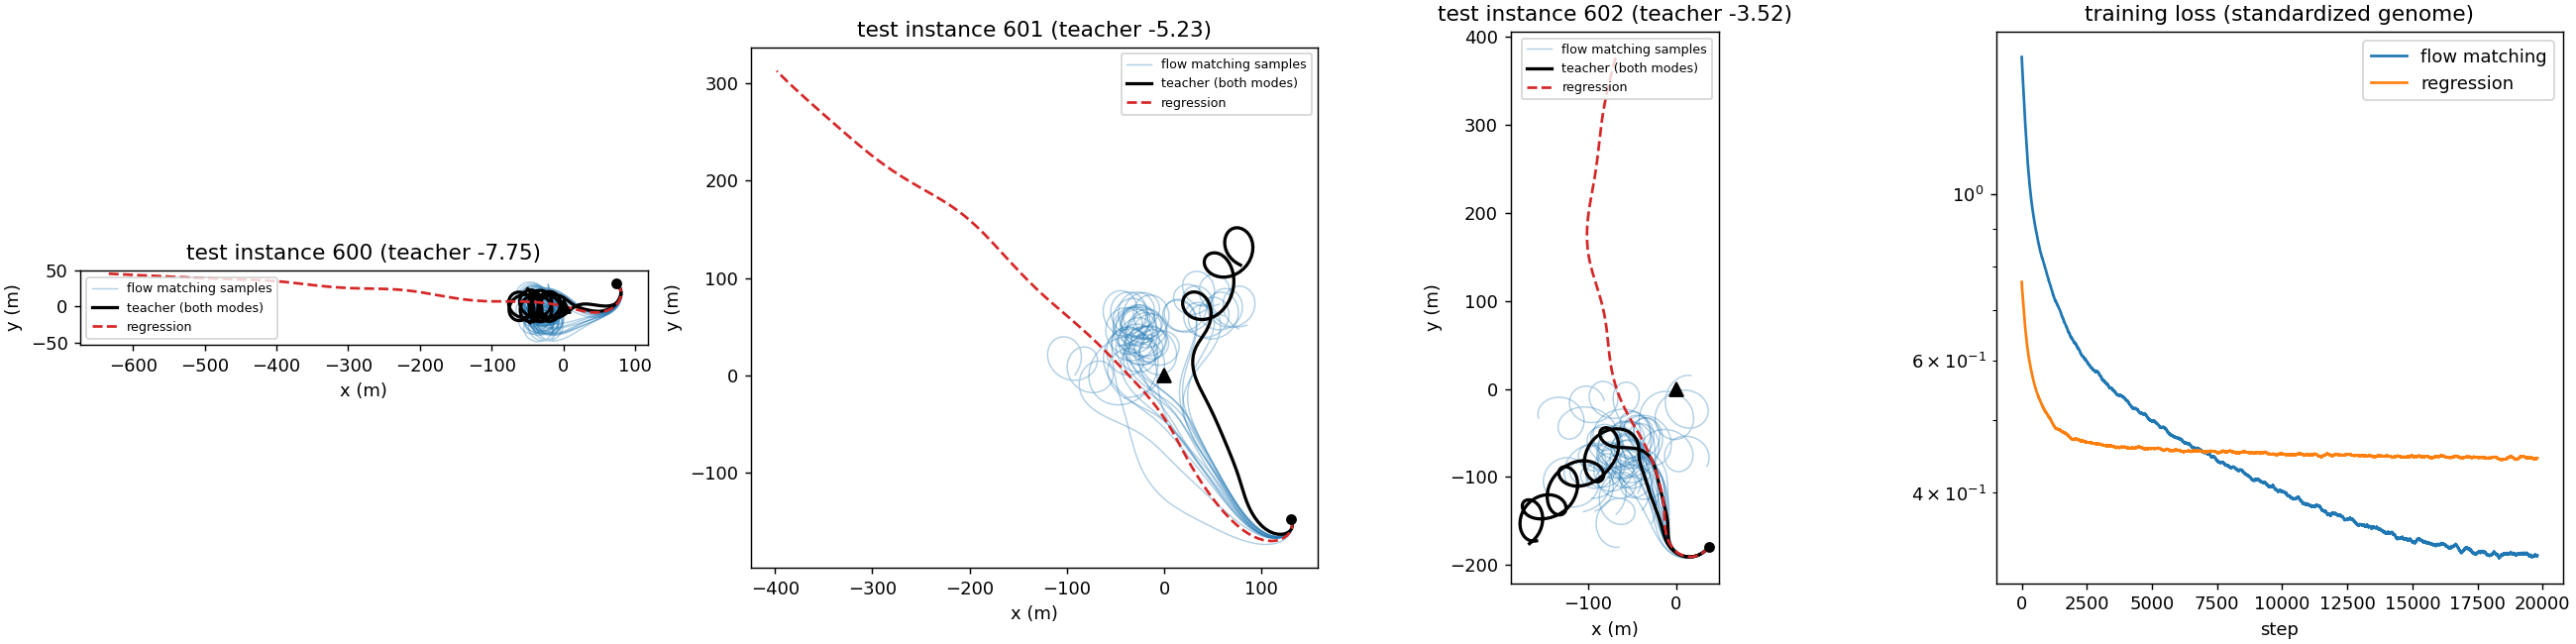
\includegraphics[width=\linewidth]{phase3_student.png}
\caption{Regression averages the two orbit directions into a straight line out of the thermal; flow matching samples circle in both directions.}\label{fig:student}
\end{figure}

\begin{figure}[ht]\centering
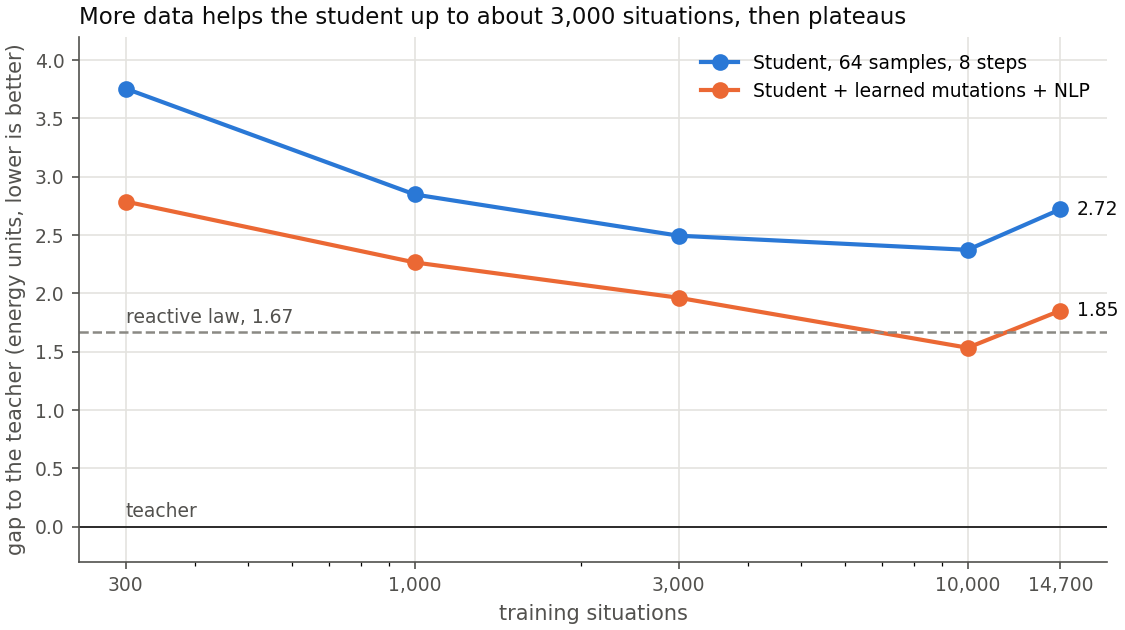
\includegraphics[width=0.62\linewidth]{savio_scaling.png}
\caption{Scaling: the student's gap to the teacher against the number of training situations. More data helps up to about 3{,}000 situations, then the limit is the model.}\label{fig:scaling}
\end{figure}

\section{The genetic algorithm in a latent space}
The phase 2 GA failed on 87 coupled genes. A conditional VAE compresses the teacher's trajectories into $d = 8$, 16 or 32 latent dimensions, and the same GA (population 50, 3{,}000 evaluations) searches that space; each individual is decoded and scored. Searching the latent space rescues the GA: 55\,\% to 100\,\% solved. But only about 20\,\% of the teacher's own trajectories survive the encode--decode round trip: small position errors become large $\CL$ and thrust errors through the flat map.

\section{A decoder that is a simulator}
\begin{figure}[ht]\centering
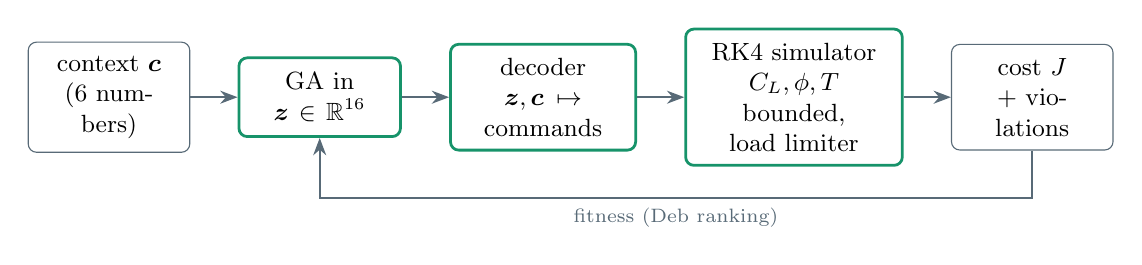
\begin{tikzpicture}[node distance=0.6cm]
  \node[blk, text width=1.7cm] (c) {context $\vect c$\\(6 numbers)};
  \node[key, text width=1.7cm, right=of c] (ga) {GA in\\$\vect z\in\R^{16}$};
  \node[key, text width=2.0cm, right=of ga] (dec) {decoder\\$\vect z,\vect c\mapsto$ commands};
  \node[key, text width=2.4cm, right=of dec] (sim) {RK4 simulator\\$\CL,\phi,T$ bounded,\\load limiter};
  \node[blk, text width=1.7cm, right=of sim] (cost) {cost $J$\\+ violations};
  \draw[arr] (c) -- (ga); \draw[arr] (ga) -- (dec); \draw[arr] (dec) -- (sim); \draw[arr] (sim) -- (cost);
  \draw[arr] (cost.south) -- ++(0,-0.6) -| node[lab, pos=0.25, below]{fitness (Deb ranking)} (ga.south);
\end{tikzpicture}
\caption{Latent search with the physics decoder: every candidate is decoded into commands and flown.}\label{fig:physdec}
\end{figure}
The decoder of the command VAE outputs \emph{commands} ($\CL$, bank, thrust at 61 knots over 60\,s) squashed into their limits, and a batched RK4 point-mass simulator (PyTorch, differentiable) turns them into the trajectory, with a load limiter that caps $\CL$ at every step. $\CL$, bank, thrust and load factor cannot be violated by construction. The VAE learns the teacher's commands read off its trajectories by the flat map. The round trip goes from 20\,\% to 100\,\% feasible, and on 77 test situations (Table~\ref{tab:physics}):

\begin{table}[ht]\centering\small
\caption{Phase 3, point-mass wing, 77 test situations (teacher $-5.24$).}\label{tab:physics}
\begin{tabular}{@{}lcccc@{}}
\toprule
Method & Solved & Cost & Gap & Time per plan \\ \midrule
GA on the 87 genes + SLSQP & 55\,\% & $+1.92$ & 7.09 & -- \\
Latent GA, position VAE + SLSQP & 100\,\% & $-3.59$ & 1.64 & -- \\
Teacher's commands, flown & 100\,\% & $-4.70$ & 0.54 & 0.14\,s \\
64 prior samples, physics VAE & 100\,\% & $-5.21$ & 0.03 & 0.2\,s \\
\textbf{Latent GA, physics VAE} & 100\,\% & $\mathbf{-6.06}$ & $\mathbf{-0.82}$ & 12.6\,s \\
\bottomrule
\end{tabular}
\end{table}

\begin{figure}[ht]\centering
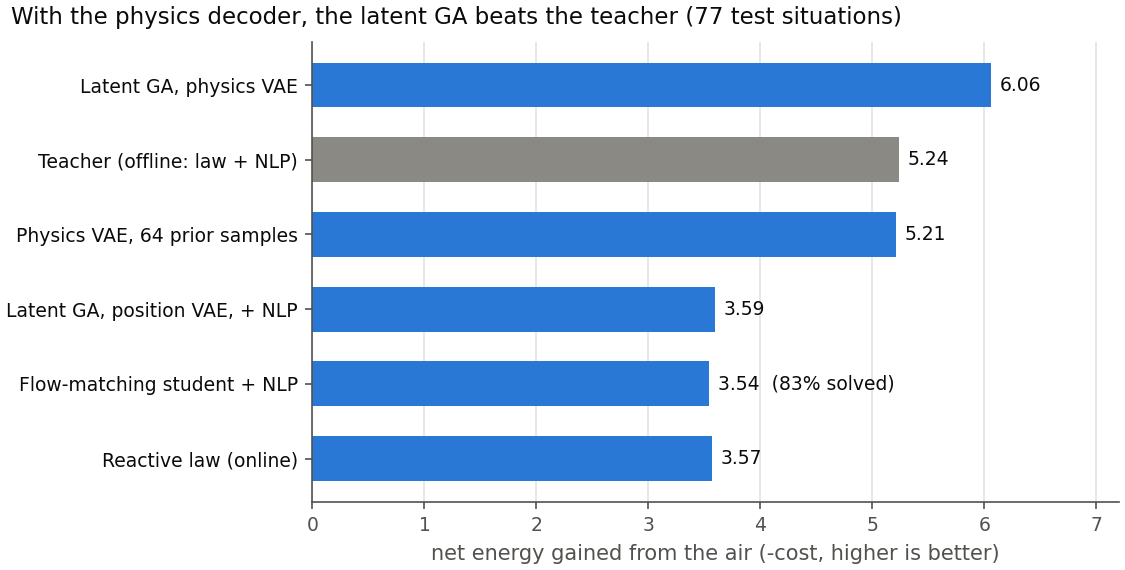
\includegraphics[width=0.66\linewidth]{savio_methods.png}
\caption{Energy gained on 77 test situations: the latent GA over the physics decoder beats the teacher.}\label{fig:methods}
\end{figure}

\section{Realism: tight turns and the strip wing}
The latent GA gained mostly by circling tighter (median radius 15--25\,m against 21--29\,m). Under a common minimum turn radius its lead shrinks (from $-0.85$ without limit to $-0.35$ at 15\,m) and reverses at 18\,m; with the strip wing applied to every method and a VAE trained on point-mass trajectories, it falls behind the teacher ($-4.28$ against $-4.70$). Regenerating the teacher with the strip wing (two seeds, 15{,}080 situations) and retraining restores the lead (Table~\ref{tab:strip}).

\begin{table}[ht]\centering\small
\caption{Strip wing, retrained, 65 test situations.}\label{tab:strip}
\begin{tabular}{@{}lccc@{}}
\toprule
Method & $d=8$ & $d=16$ & $d=32$ \\ \midrule
Teacher & $-4.88$ & $-4.88$ & $-4.88$ \\
Teacher's commands, flown & $-4.45$ & $-4.45$ & $-4.45$ \\
64 prior samples & $-4.72$ & $-4.64$ & $-4.65$ \\
\textbf{Latent GA} & $-5.37$ & $-5.69$ & $\mathbf{-5.72}$ \\
\bottomrule
\end{tabular}
\end{table}

\section{Sensitivity to the estimated polar}\label{sec:sensitivity}
Scaling $C_{D0}$, $\CLmax$ or the mass by 0.8 or 1.2 for every method (Table~\ref{tab:sens}): drag moves everything by about 0.5 and leaves the gap at $-0.8$; the stall margin governs the lead. A heavier airframe or a lower $\CLmax$ flies closer to stall and the lead shrinks to $-0.1$ (still positive); without search the prior does not transfer to another airframe.

\begin{table}[ht]\centering\small
\caption{Sensitivity to the SB-XC's estimated polar (65 situations, $d=16$).}\label{tab:sens}
\begin{tabular}{@{}lcccc@{}}
\toprule
Airframe & Teacher (solved) & Prior & Latent GA & Gap \\ \midrule
nominal & $-4.91$ (100\,\%) & $-4.64$ & $-5.69$ & $-0.79$ \\
$C_{D0}\times0.8$ & $-5.48$ (100\,\%) & $-5.13$ & $-6.29$ & $-0.81$ \\
$C_{D0}\times1.2$ & $-4.44$ (100\,\%) & $-4.24$ & $-5.23$ & $-0.79$ \\
$\CLmax\times1.2$ & $-5.30$ (100\,\%) & $-5.29$ & $-6.24$ & $-0.94$ \\
mass $\times0.8$ & $-5.70$ (100\,\%) & $-5.57$ & $-6.93$ & $-1.23$ \\
$\CLmax\times0.8$ & $-4.11$ (89\,\%) & $-2.53$ & $-4.49$ & $-0.09$ \\
mass $\times1.2$ & $-4.36$ (100\,\%) & $-2.81$ & $-4.49$ & $-0.13$ \\
\bottomrule
\end{tabular}
\end{table}

%=====================================================================
\chapter{Closed-loop flight}\label{ch:closedloop}

\section{Air, belief and autopilot}
Until here every planner was scored in the air it planned in. In closed loop the two part (Fig.~\ref{fig:loop}): the \emph{air} is the situation with the strip wing plus Dryden turbulence; the planner has a \emph{belief} of the thermal's centre, strength and wind, off by sampled errors. A path tracker (the autopilot) follows the plan as a path, not a clock: at each step it finds the closest reference point ahead and commands
\begin{equation}
\vect a_c = \vect a_r + k_v\,\vect e_v^\perp + k_p\,\vect e_p^\perp + \big(k_z e_z + k_V (V_a - V_{a,r})\big)\hat{\vect e}_z,
\end{equation}
turned into $\CL$ and bank by the flat map, through a first-order attitude lag (0.3\,s), a bank-rate limit, a $\CL$ protection at 90\,\% of $\CLmax$, bank $\le 40^\circ$, the motor and the aileron drag.

\begin{figure}[ht]\centering
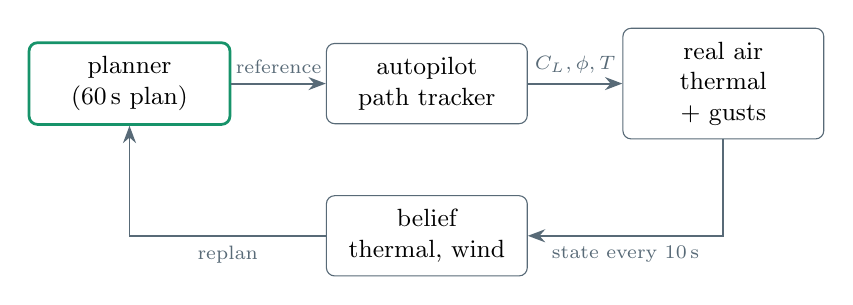
\begin{tikzpicture}[node distance=0.7cm]
  \node[key, text width=2.2cm] (plan) {planner\\(60\,s plan)};
  \node[blk, text width=2.2cm, right=1.2cm of plan] (track) {autopilot\\path tracker};
  \node[blk, text width=2.2cm, right=1.2cm of track] (air) {real air\\thermal + gusts};
  \node[blk, text width=2.2cm, below=0.9cm of track] (bel) {belief\\thermal, wind};
  \draw[arr] (plan) -- node[lab, above]{reference} (track);
  \draw[arr] (track) -- node[lab, above]{$\CL,\phi,T$} (air);
  \draw[arr] (air.south) |- node[lab, pos=0.75, below]{state every 10\,s} (bel.east);
  \draw[arr] (bel.west) -| node[lab, pos=0.25, below]{replan} (plan.south);
\end{tikzpicture}
\caption{Closed loop: plan in the belief, fly in the real air, replan every 10\,s from the state reached.}\label{fig:loop}
\end{figure}

\section{Making replanning safe}
Replanning every 10\,s with a planner that scores a fixed 60\,s window failed: every plan put its energy gain at the end of its window, and the next replanning pushed that gain away (on one situation, $-3.47$ replanned against $-7.11$ open loop, with the first 10\,s of every plan flown exactly as predicted). The fix is a \emph{shrinking horizon}: a plan made at time $t_0$ of a flight of duration $T_f$ minimizes
\begin{equation}
J_{t_0} = J\big(\vect p_{[t_0,\,T_f]}\big),
\end{equation}
the cost up to the flight's end, so that replanning optimizes the objective that is scored. Every plan also starts from the state reached (velocity, acceleration, $\CL$, bank, thrust), keeps the orbit direction already taken, is warm-started from the rest of the plan being flown, and has that rest as a candidate: in its belief a new plan is never worse than carrying on.

\section{Results}
\begin{figure}[ht]\centering
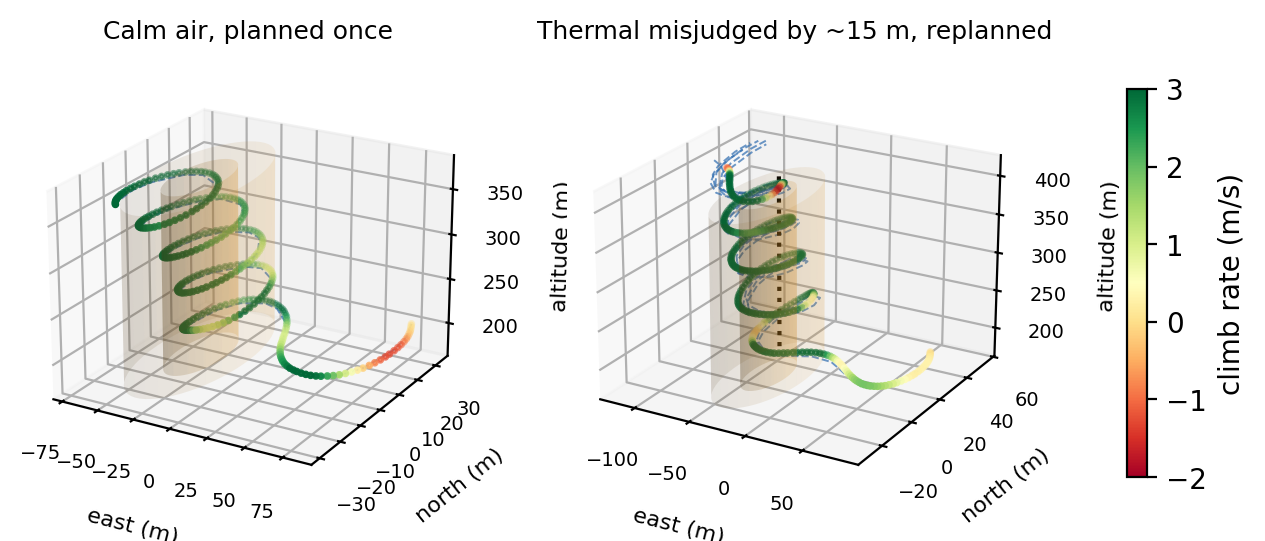
\includegraphics[width=0.95\linewidth]{flight60_3d.png}
\caption{Two 60\,s flights in 3D, coloured by climb rate; orange: thermal core (15 and 30\,m), blue dashes: plans, dotted: believed centre. Right: the spiral is clean but off-centre.}\label{fig:flight3d}
\end{figure}

\begin{table}[ht]\centering\small
\caption{Closed loop, Savio: 65 situations $\times$ 4 conditions, replanned every 10\,s (no inner-wing limiter yet).}\label{tab:closedloop}
\begin{tabular}{@{}llccc@{}}
\toprule
Condition & Planner & Flown cost & Without violation & Stalled \\ \midrule
calm & teacher & $-4.69$ & 92\,\% & 3\,\% \\
     & latent GA & $\mathbf{-5.41}$ & 55\,\% & 11\,\% \\
     & VAE prior & $-4.56$ & 86\,\% & 3\,\% \\ \midrule
turbulence & teacher & $-4.15$ & 25\,\% & 52\,\% \\
           & latent GA & $-4.78$ & 2\,\% & 92\,\% \\ \midrule
wrong belief & teacher & $-2.03$ & 37\,\% & 35\,\% \\
             & latent GA & $-1.87$ & 3\,\% & 85\,\% \\ \midrule
both & teacher & $-1.87$ & 3\,\% & 85\,\% \\
     & latent GA & $-1.64$ & 2\,\% & 97\,\% \\
\bottomrule
\end{tabular}
\end{table}

The autopilot tracks plans within 1--2\,m on average (6.6\,m at worst in gusts). In calm air the latent GA keeps its lead and replanning does at least as well as the open loop. A wrong belief (centre off by 15\,m per axis, $w^\star$ by 20\,\%, wind by 0.5\,m/s) costs more than everything else: every method falls to about $-2$, and replanning cannot help while the belief is not corrected (Fig.~\ref{fig:flight3d}). Gusts make the inner wing stall: the plans use the whole stall margin.

%=====================================================================
\chapter{Cross-country flight}\label{ch:xc}

\section{Tasks}
A task sends the aircraft to a goal 20\,km away through a Poisson field of drifting thermals (about one per km\textsuperscript{2} over a 2\,km corridor, $w^\star\in[1.2,2.8]$\,m/s), from 250--350\,m, with a cloud base at 600\,m and the motor allowed below 120\,m. The score is equation~\eqref{eq:cost} over the whole flight with $E_{\mathrm{ref}}$ the battery energy of the same distance on the motor (the motor scores about 1).

\section{A two-level pilot}
\begin{figure}[ht]\centering
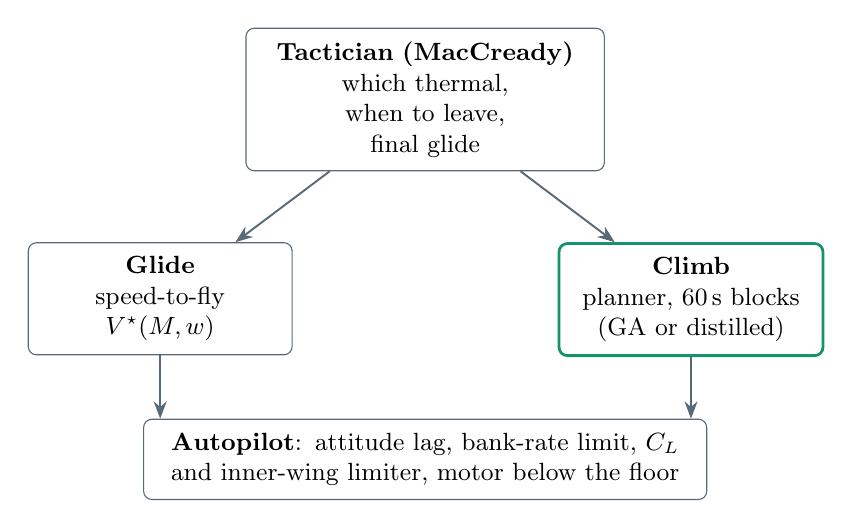
\begin{tikzpicture}[node distance=0.5cm]
  \node[blk, text width=4.2cm] (tac) {\textbf{Tactician (MacCready)}\\which thermal, when to leave,\\final glide};
  \node[blk, text width=3.0cm, below left=0.9cm and -0.6cm of tac] (glide) {\textbf{Glide}\\speed-to-fly $V^\star(M,w)$};
  \node[key, text width=3.0cm, below right=0.9cm and -0.6cm of tac] (climb) {\textbf{Climb}\\planner, 60\,s blocks\\(GA or distilled)};
  \node[blk, text width=6.8cm] (ap) at ($(tac.south |- climb.south) + (0,-1.3)$) {\textbf{Autopilot}: attitude lag, bank-rate limit, $\CL$ and inner-wing limiter, motor below the floor};
  \draw[arr] (tac) -- (glide); \draw[arr] (tac) -- (climb);
  \draw[arr] (glide) -- (ap.north -| glide); \draw[arr] (climb) -- (ap.north -| climb);
\end{tikzpicture}
\caption{The cross-country pilot: a rule-based tactician over glide and climb modes, and the autopilot underneath.}\label{fig:xcpilot}
\end{figure}

The tactician chooses, among the thermals reachable with an arrival margin of 60\,m above the floor, the one with the best rate of progress toward the goal, counting the time to climb back the height the glide costs:
\begin{equation}
i^\star = \arg\max_i \frac{\Delta_i}{d_i/V^\star + (d_i/(L/D)^\star)/c_i},
\end{equation}
with $\Delta_i$ the progress toward the goal, $d_i$ the distance to thermal $i$, $(L/D)^\star$ the glide ratio at the speed-to-fly and $c_i$ the expected climb rate. It leaves a thermal once the climb averaged over 20\,s falls below $M$ or at the cloud base, and starts the final glide when it is safe. Climbs are flown either by a circling rule or by a planner in 60\,s blocks (motor off), cut at the cloud base.

\section{An inner-wing limiter}
The first 64-task run showed the latent GA climbing 60\,\% faster but stalling a wing section in 19 to 69\,\% of its flights. A limiter in the autopilot caps the $\CL$ command so that no strip passes a fraction $f = 0.9$ of its section stall, before and after the attitude lag:
\begin{equation}
\CL^{\mathrm{cmd}} \le \frac{f\,c_{\ell,\max}}{\max_y c_\ell(y)/\CL}\bigg|_{V_a,\,\phi},
\end{equation}
the ratio of the local peak to the mean $\CL$ being given by strip theory at the current airspeed and bank.

\section{Results}
\begin{figure}[ht]\centering
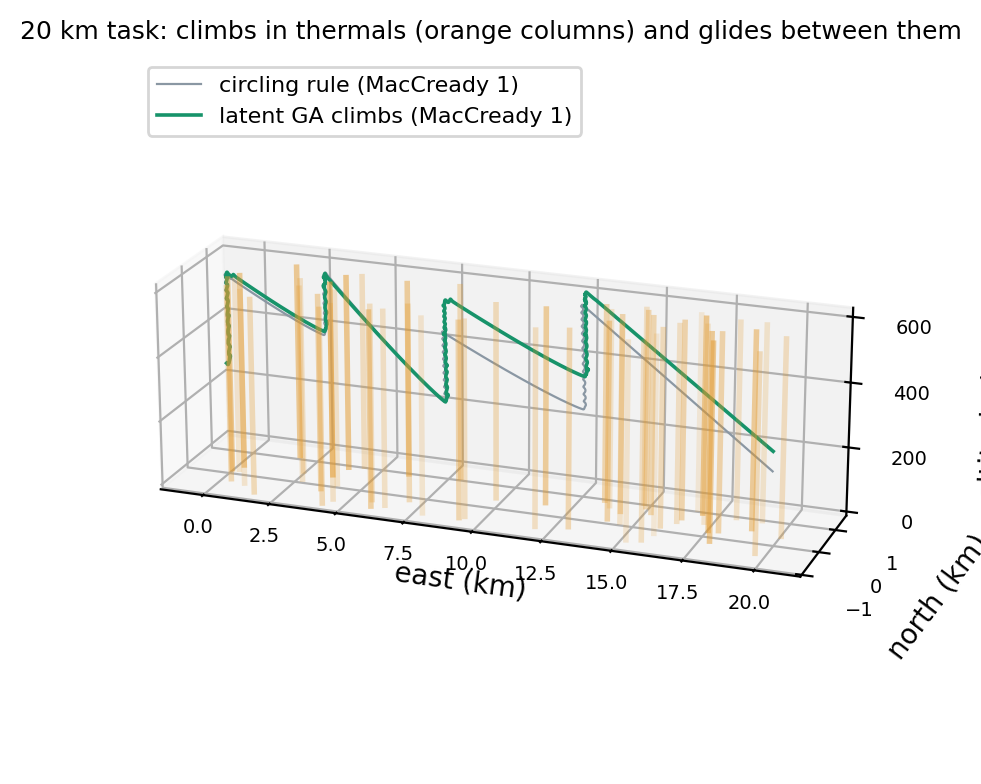
\includegraphics[width=\linewidth]{xc_3d.png}
\caption{A 20\,km task in 3D: thermals as columns, climbs and glides of two pilots (vertical axis: altitude in m).}\label{fig:xc3d}
\end{figure}

\begin{figure}[ht]\centering
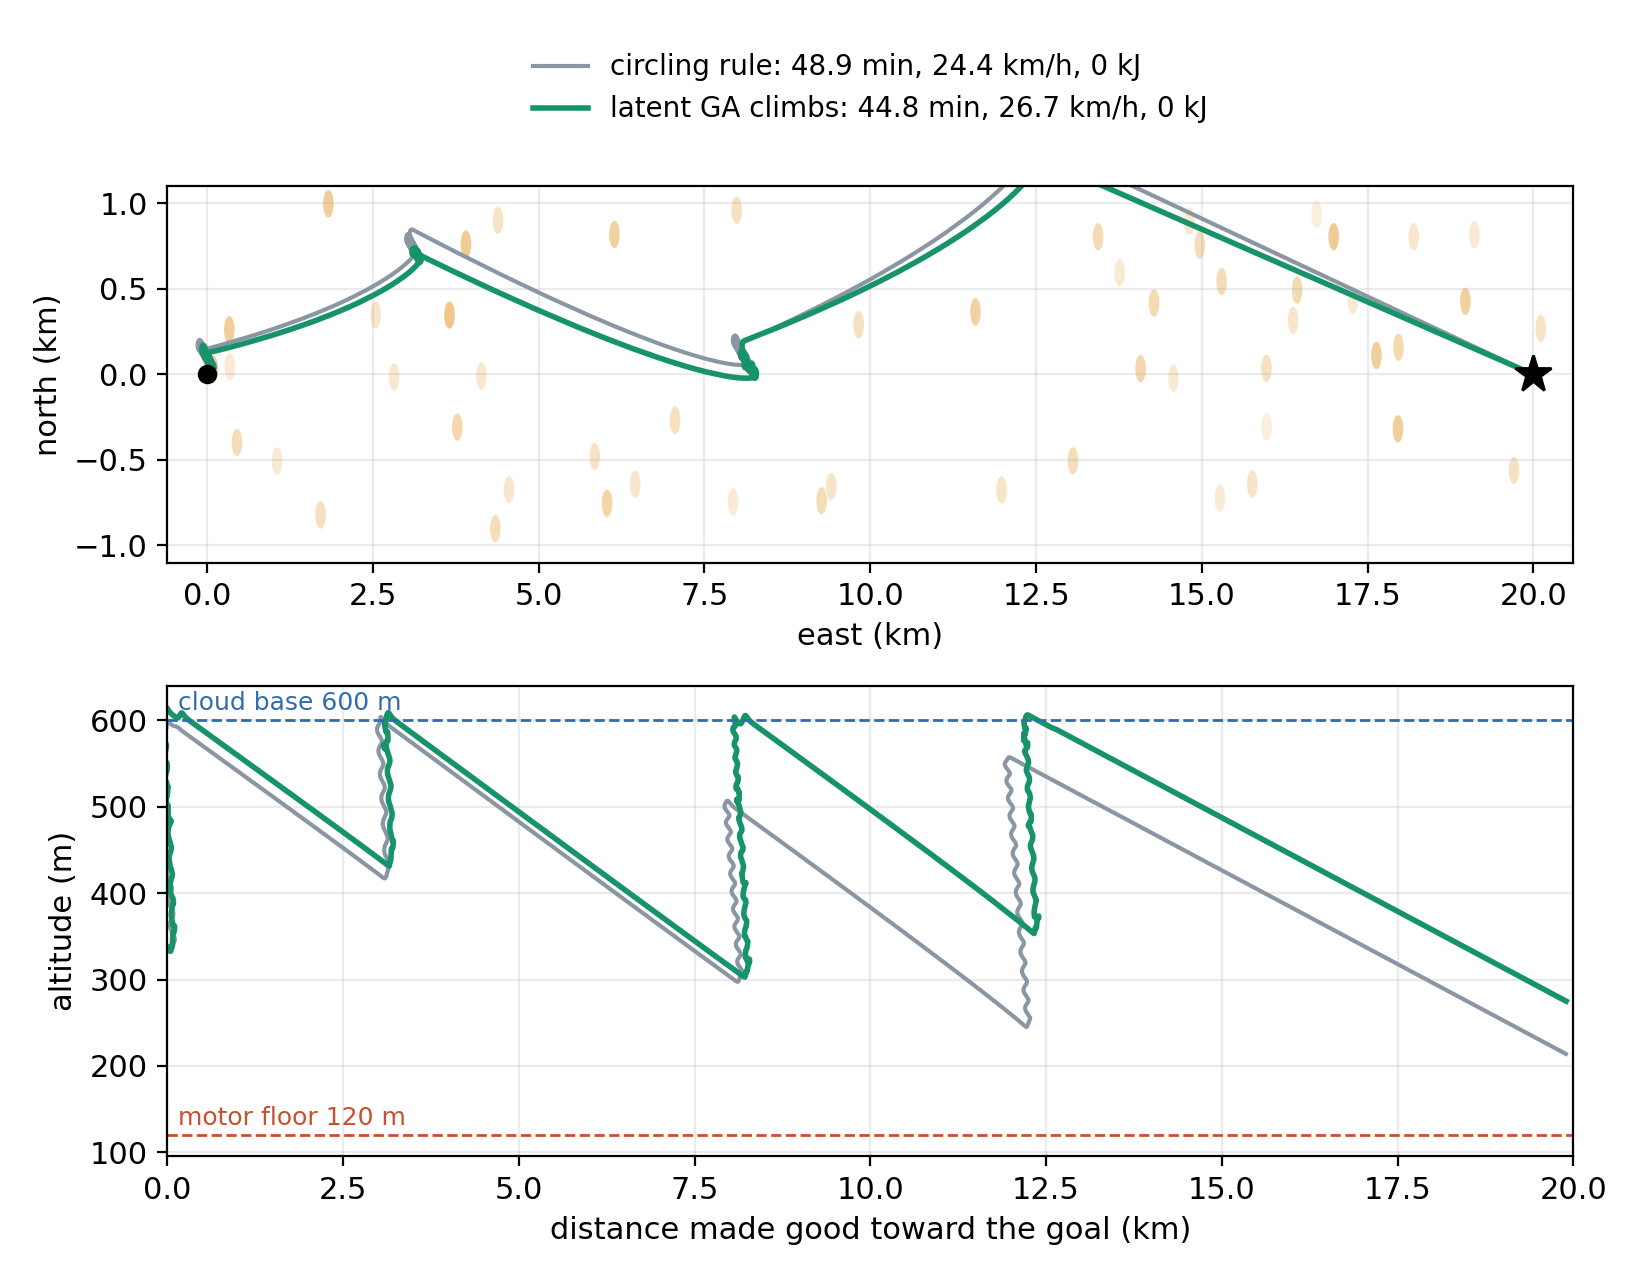
\includegraphics[width=0.85\linewidth]{xc_flight_en.png}
\caption{The same task: top view and barogram (altitude against distance toward the goal).}\label{fig:baro}
\end{figure}

\begin{table}[ht]\centering\small
\caption{64 tasks of 20\,km, protected autopilot for every pilot.}\label{tab:xc}
\resizebox{\linewidth}{!}{\begin{tabular}{@{}lccccc@{}}
\toprule
Pilot & Battery & Speed & Mean climb & Stalled & No violation \\ \midrule
Motor all the way & 61.9\,kJ & 29.2\,km/h & -- & 0\,\% & 100\,\% \\
Circling rule, MacCready 0.5 & 2.9\,kJ & 24.9\,km/h & 1.29\,m/s & 0\,\% & 100\,\% \\
Circling rule, MacCready 1 & 19.3\,kJ & 28.3\,km/h & 1.22\,m/s & 0\,\% & 100\,\% \\
\textbf{Latent GA climbs, MacCready 0.5} & 2.9\,kJ & \textbf{28.2\,km/h} & \textbf{2.08\,m/s} & 0\,\% & 98\,\% \\
\textbf{Latent GA climbs, MacCready 1} & 4.7\,kJ & \textbf{29.5\,km/h} & \textbf{2.07\,m/s} & 0\,\% & 100\,\% \\
GA with a 20\,\% stall margin, MacCready 1 & 4.7\,kJ & 29.0\,km/h & 1.90\,m/s & 0\,\% & 100\,\% \\
\bottomrule
\end{tabular}}
\end{table}

The latent GA climbs 61\,\% faster than the circling rule; at the same setting the flight is 3.3\,km/h faster on the same battery (faster on 89\,\% of the tasks), and at MacCready 1 it matches the motor's speed on 13 times less battery. The limiter removes every stall without reducing the lead (2.08 against 2.09\,m/s): the gain did not come from flying at the stall. A stall margin in the plan is also safe but costs 6--8\,\% of the climb.

%=====================================================================
\chapter{Distilling the search}\label{ch:distill}

\section{Distillation}
\begin{figure}[ht]\centering
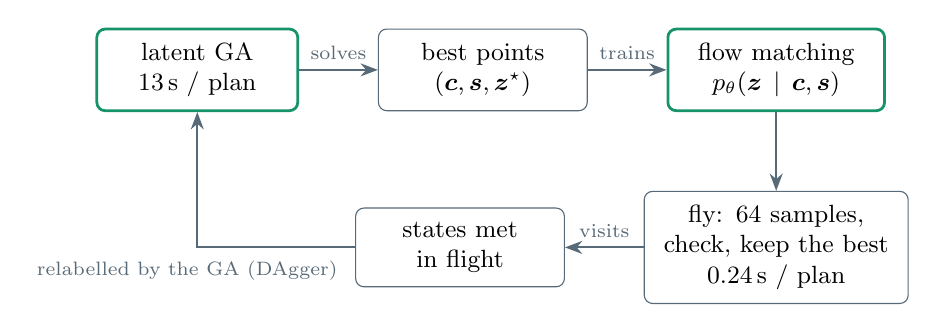
\begin{tikzpicture}[node distance=0.6cm]
  \node[key, text width=2.2cm] (ga) {latent GA\\13\,s / plan};
  \node[blk, text width=2.3cm, right=1.0cm of ga] (data) {best points\\$(\vect c, \vect s, \vect z^\star)$};
  \node[key, text width=2.4cm, right=1.0cm of data] (fm) {flow matching\\$p_\theta(\vect z\mid\vect c,\vect s)$};
  \node[blk, text width=3.0cm, below=1.0cm of fm] (fly) {fly: 64 samples,\\check, keep the best\\0.24\,s / plan};
  \node[blk, text width=2.3cm, left=1.0cm of fly] (states) {states met\\in flight};
  \draw[arr] (ga) -- node[lab, above]{solves} (data);
  \draw[arr] (data) -- node[lab, above]{trains} (fm);
  \draw[arr] (fm) -- (fly);
  \draw[arr] (fly) -- node[lab, above]{visits} (states);
  \draw[arr] (states.west) -| (ga.south);
  \node[lab, anchor=north east] at ($(states.west)+(-0.1,-0.05)$) {relabelled by the GA (DAgger)};
\end{tikzpicture}
\caption{Distillation of the search and the DAgger loop.}\label{fig:dagger}
\end{figure}

The latent GA solves 3{,}000 training situations and keeps its best point $\vect z^\star$ in the command VAE's latent box; a conditional flow-matching model learns $p_\theta(\vect z\mid\vect c)$ from those points (equation~\eqref{eq:fm}, MLP $3\times256$). In flight, 64 samples are decoded, flown in the belief and the best is kept (Table~\ref{tab:distill}). The generator matches the GA at 57 times less compute and beats the teacher by 0.85; one sample is not enough, and a short search on top adds nothing.

\begin{table}[ht]\centering\small
\caption{Distillation, 65 test situations (teacher $-4.88$).}\label{tab:distill}
\begin{tabular}{@{}lcccc@{}}
\toprule
Method & Solved & Cost & Gap & Time per plan \\ \midrule
64 samples of the VAE prior & 100\,\% & $-4.64$ & $+0.24$ & 0.24\,s \\
1 sample of the distilled generator & 94\,\% & $-3.52$ & $+1.30$ & 0.14\,s \\
\textbf{64 samples of the distilled generator} & 100\,\% & $\mathbf{-5.72}$ & $\mathbf{-0.85}$ & \textbf{0.24\,s} \\
Distilled samples + a short GA (300 flights) & 100\,\% & $-5.59$ & $-0.71$ & 1.4\,s \\
Latent GA (3{,}000 flights), the target & 100\,\% & $-5.66$ & $-0.78$ & 13.4\,s \\
\bottomrule
\end{tabular}
\end{table}

\section{A DAgger round}
Flown on the 20\,km tasks, that generator kept little of the GA's lead (Table~\ref{tab:dagger}): it had learned level starts at 180--320\,m, while a climb is replanned in a turn, up to 600\,m, and its condition did not hold the current bank. Following DAgger, the GA flew the tasks with every climb plan it won recorded (1{,}095 plans: situation, aircraft state $\vect s = (\phi, V_a, \CL)$, latent point), and the generator was retrained on those plus the 3{,}000 situations of the first round, conditioned on $(\vect c, \vect s)$.

\begin{table}[ht]\centering\small
\caption{64 tasks of 20\,km, MacCready 0.5 / 1.}\label{tab:dagger}
\resizebox{\linewidth}{!}{\begin{tabular}{@{}lcccc@{}}
\toprule
Climbs & Mean climb & Speed & Battery & Time per plan \\ \midrule
Circling rule & 1.29 / 1.22\,m/s & 24.9 / 28.3\,km/h & 2.9 / 19.3\,kJ & feedback \\
Latent GA & 2.08 / 2.07\,m/s & 28.2 / 29.5\,km/h & 2.9 / 4.7\,kJ & $\approx$13\,s \\
Generator distilled on S1 only & 1.50 / 1.17\,m/s & 25.1 / 28.8\,km/h & 4.2 / 20.2\,kJ & 0.24\,s \\
\textbf{Generator after one DAgger round} & \textbf{2.23 / 2.20\,m/s} & \textbf{28.5 / 30.2\,km/h} & 2.9 / 4.7\,kJ & \textbf{0.24\,s} \\
\bottomrule
\end{tabular}}
\end{table}

After one round the generator climbs as fast as the GA it imitates and slightly faster (faster on 84\,\% and 77\,\% of the tasks), likely because it draws 64 verified candidates from thousands of GA solutions while the GA has 1{,}000 flights per plan in flight. At MacCready 1 it beats the motor's speed (30.2 against 29.2\,km/h) on 13 times less battery, with no stall, and it is unchanged on the S1 test situations.

\begin{figure}[ht]\centering
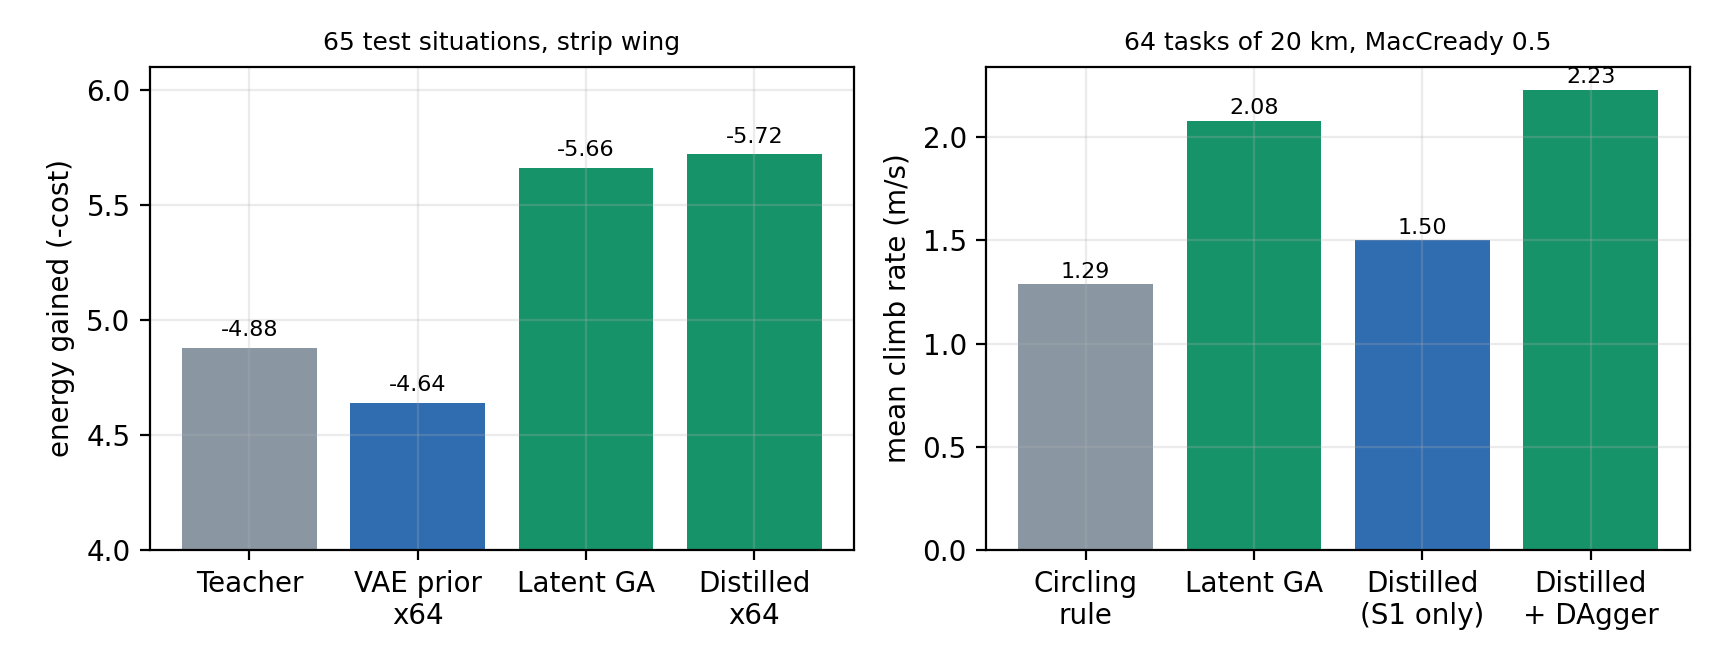
\includegraphics[width=0.92\linewidth]{summary_bars.png}
\caption{Summary. Left: energy gained on 65 test situations. Right: mean climb rate on 64 tasks of 20\,km.}\label{fig:summary}
\end{figure}

%=====================================================================
\chapter{Discussion}\label{ch:discussion}

\section{What the results show}
\begin{enumerate}
  \item \textbf{Representation decides whether evolutionary search works.} The same GA is the weakest optimizer on 87 coupled genes and the best method in a 16-dimensional learned space, beating the teacher that produced the data.
  \item \textbf{Physics belongs in the decoder.} Decoding into bounded commands flown by a simulator turns feasibility from 20\,\% to 100\,\%.
  \item \textbf{The binding limit of a circling sailplane is inner-wing stall}, not the turn radius; the cure is a faster orbit, and the stall margin (wing loading, $\CLmax$), not drag, governs the gain.
  \item \textbf{Receding horizons procrastinate} under a terminal-energy objective; plans must aim at the flight's end.
  \item \textbf{Knowing where the thermal is matters more than planning well}: 15\,m of error cost more than turbulence.
  \item \textbf{Safety belongs in the autopilot}: a stall limiter costs nothing, a margin in the plan costs climb.
  \item \textbf{Search can be distilled}, provided the generator is shown the states met in flight.
\end{enumerate}

\section{Between MPC and reinforcement learning}
The final system is an amortized model-predictive controller: a learned proposal distribution replaces most of the online optimization, and a physics check keeps every plan honest. A GA over trajectories is planning (the MPC side); a GA over the 10 parameters of the reactive law is policy search (the reinforcement-learning side). The distilled generator sits between them: it is trained offline on search outputs like a policy, and used online as a sampler inside a planner.

\section{Threats to validity}
\begin{itemize}
  \item Simulation only: a 3-DOF point mass with a strip-theory wing and an attitude lag, not 6-DOF.
  \item A synthetic thermal model; in the cross-country tasks the thermals are known exactly.
  \item One run per configuration for the Savio benchmarks (64--80 tasks each, paired comparisons).
  \item 17\,\% of the S1 situations are left unsolved by the teacher and excluded from the tests.
  \item The SB-XC's polar is estimated (tested at $\pm$20\,\%).
\end{itemize}

%=====================================================================
\chapter{Towards a flight test}\label{ch:towards}

\section{Target platform}
The longer-term goal is to test the approach on one of the laboratory's airframes. The exact platform is to be confirmed with the laboratory (exchange with Jay); the sensitivity study tells what must be measured first: wing loading and $\CLmax$, the parameters that govern the gain, before the drag polar.

\section{Estimating the thermal in flight}
The largest measured loss comes from the belief. The next step is an onboard estimator that recentres the thermal from the aircraft's own vario, in the spirit of ArduPilot's soaring controller: with $\hat w(t)$ the measured netto (air-mass vertical speed, from total-energy rate plus the polar's sink rate), a parametric thermal $w(\vect p; \vect\theta)$ with $\vect\theta = (x_c, y_c, w_{\mathrm{peak}}, r)$ is fitted by an extended Kalman filter,
\begin{equation}
\hat{\vect\theta}_{k+1} = \hat{\vect\theta}_k + K_k\big(\hat w_k - w(\vect p_k;\hat{\vect\theta}_k)\big),
\end{equation}
and the replanning uses the updated belief. Circling gives the filter the radial excitation it needs: the climb is stronger on the side closer to the core.

\section{Integration}
\begin{itemize}
  \item \textbf{Software in the loop}: the planner (0.24\,s per plan on one server core) inside PX4 or ArduPilot SITL, flying the existing autopilot loops.
  \item \textbf{Onboard compute}: the generator's 64 samples and their simulation are batched; an embedded GPU (e.g.\ Jetson class) should bring a plan well under the 10\,s replanning period.
  \item \textbf{Retraining}: a teacher dataset and a command VAE for the identified airframe, then the DAgger round on its own flight states.
\end{itemize}

%=====================================================================
\chapter{Conclusion}\label{ch:conclusion}
Planning to soar is a hard, multimodal, constraint-bound problem. Searching the right space turned a failing genetic algorithm into a planner that beats the optimizer that taught it; putting the physics in the decoder made every proposal feasible; flying the plans in closed loop showed that knowing where the thermal is now matters more than planning well; and distilling the search, then correcting it on the states met in flight, gave a planner that runs in a quarter of a second with the quality of the search. On 64 tasks of 20\,km it climbs 70\,\% faster than a classic circling rule, matches motorized flight on 13 times less battery, and does not stall. The next steps are an onboard thermal estimator and a flight test on a laboratory airframe.

%=====================================================================
\appendix
\chapter{Reproducibility}
All code is public at \url{https://github.com/clementdumeril/GeneticWing}. The main commands (Savio, from the repository root) are:
\begin{itemize}
  \item \texttt{bash slurm/submit\_all.sh strip}: teacher on 15{,}080 situations, merge, physics study;
  \item \texttt{bash slurm/submit\_all.sh sensitivity}, \texttt{closedloop}, \texttt{xc}, \texttt{distill}, \texttt{dagger}: the studies of Chapters~\ref{ch:student}--\ref{ch:distill};
  \item \texttt{python scenarios/phase4\_view.py}, \texttt{phase5\_view.py}: self-contained 3D pages of flights.
\end{itemize}
Compute: Savio (UC Berkeley) CPU nodes of 32 cores and A40 GPUs; two desktop machines (i7-3770, i5-6500) for smaller runs. The software uses NumPy, SciPy and PyTorch, with 69 unit tests.

\chapter{Main hyperparameters}
\begin{table}[ht]\centering\small
\caption{Main hyperparameters.}\label{tab:hyper}
\begin{tabular}{@{}ll@{}}
\toprule
Genome & B-spline degree 5, 32 control points, 87 genes \\
Teacher & law seeds (tuned, faster orbit) $\times$ 2 directions, SLSQP 6{,}000 evaluations, margins \\
GA & real-coded, population 50, SBX + polynomial mutation, Deb ranking \\
Latent GA & 3{,}000 flights (1{,}000 in the cross-country climbs) \\
Command VAE & 61 knots $\times$ 3 commands, latent $d=16$, $\beta = 0.1$, MLP $3\times512$, 20{,}000 steps \\
Flow matching & MLP $3\times256$ (latent) or $4\times512$ (genomes), 20{,}000 steps, 8 Euler steps \\
Simulator & RK4, 0.4\,s steps (plans), 0.02\,s (tracker) \\
Closed loop & 60\,s flights, replanning every 10\,s, shrinking horizon \\
Cross-country & 20\,km, cloud base 600\,m, motor floor 120\,m, climbs in 60\,s blocks \\
Limiter & every wing section below 90\,\% of its stall \\
\bottomrule
\end{tabular}
\end{table}

\begin{thebibliography}{99}
\bibitem{allen2006} M.~J. Allen, ``Updraft model for development of autonomous soaring uninhabited air vehicles,'' AIAA Aerospace Sciences Meeting, AIAA 2006-1510, 2006.
\bibitem{anthony2017} T.~Anthony, Z.~Tian, D.~Barber, ``Thinking fast and slow with deep learning and tree search,'' NeurIPS, 2017.
\bibitem{deb1995} K.~Deb, R.~B. Agrawal, ``Simulated binary crossover for continuous search space,'' Complex Systems, 9(2), 1995.
\bibitem{deb2000} K.~Deb, ``An efficient constraint handling method for genetic algorithms,'' Computer Methods in Applied Mechanics and Engineering, 186, 2000.
\bibitem{edwards2008} D.~J. Edwards, ``Implementation details and flight test results of an autonomous soaring controller,'' AIAA Guidance, Navigation and Control Conference, 2008.
\bibitem{gaier2020} A.~Gaier, A.~Asteroth, J.-B. Mouret, ``Discovering representations for black-box optimization,'' GECCO, 2020.
\bibitem{hansen2001} N.~Hansen, A.~Ostermeier, ``Completely derandomized self-adaptation in evolution strategies,'' Evolutionary Computation, 9(2), 2001.
\bibitem{kingma2014} D.~P. Kingma, M.~Welling, ``Auto-encoding variational Bayes,'' ICLR, 2014.
\bibitem{kraft1988} D.~Kraft, ``A software package for sequential quadratic programming,'' DFVLR-FB 88-28, 1988.
\bibitem{ks1979} G.~Kreisselmeier, R.~Steinhauser, ``Systematic control design by optimizing a vector performance index,'' IFAC Symposium on Computer-Aided Design of Control Systems, 1979.
\bibitem{lipman2023} Y.~Lipman, R.~T.~Q. Chen, H.~Ben-Hamu, M.~Nickel, M.~Le, ``Flow matching for generative modeling,'' ICLR, 2023.
\bibitem{liu2023} X.~Liu, C.~Gong, Q.~Liu, ``Flow straight and fast: learning to generate and transfer data with rectified flow,'' ICLR, 2023.
\bibitem{maccready1958} P.~B. MacCready, ``Optimum airspeed selector,'' Soaring, 1958.
\bibitem{milf8785c} U.S. Department of Defense, MIL-F-8785C, ``Flying qualities of piloted airplanes,'' 1980.
\bibitem{morando2025} L.~Morando et al., ``Trajectory planning and control for differentially flat fixed-wing aerial systems,'' ICRA, 2025 (arXiv:2502.00581).
\bibitem{morando2026} L.~Morando, S.~Bobbili, C.~Masci, G.~Loianno, ``Wind-aware optimal trajectory planning for efficient gliding of fixed-wing aerial systems,'' arXiv:2605.15619, 2026.
\bibitem{ross2011} S.~Ross, G.~J. Gordon, J.~A. Bagnell, ``A reduction of imitation learning and structured prediction to no-regret online learning,'' AISTATS, 2011.
\bibitem{silver2018} D.~Silver et al., ``A general reinforcement learning algorithm that masters chess, shogi, and Go through self-play,'' Science, 362, 2018.
\bibitem{volz2018} V.~Volz, J.~Schrum, J.~Liu, S.~M. Lucas, A.~Smith, S.~Risi, ``Evolving Mario levels in the latent space of a deep convolutional generative adversarial network,'' GECCO, 2018.
\end{thebibliography}

\end{document}
